%% chapter14_feature_reinforcement_learning_slides.tex
%% Beamer slides for Chapter 14: Feature Reinforcement Learning
%% An Introduction to Universal Artificial Intelligence (2024)
%% Hutter, Quarel, Catt -- Taylor & Francis / CRC Press
%% Reader-friendly style: complete sentences, symbol explanations, worked examples
%% Compiled with: pdflatex -interaction=nonstopmode chapter14_feature_reinforcement_learning_slides.tex  (twice)
\documentclass[aspectratio=169,10pt]{beamer}

\usetheme{Madrid}
\usecolortheme{seahorse}

%% ── Packages ──────────────────────────────────────────────────────────────
\usepackage{amsmath,amssymb,amsfonts}
\usepackage{mathtools}
\usepackage{graphicx}
\usepackage{booktabs}
\usepackage{xcolor}
\usepackage{listings}
\usepackage{tikz}
\usetikzlibrary{arrows.meta,positioning,shapes.geometric,fit,backgrounds}
\usepackage{algorithm}
\usepackage{algpseudocode}

\graphicspath{{figures/}}

%% ── Python listing style ─────────────────────────────────────────────────
\lstdefinestyle{pycode}{
  language=Python,
  basicstyle=\ttfamily\scriptsize,
  numbers=left,
  numberstyle=\tiny\color{gray},
  frame=single,
  backgroundcolor=\color{gray!7},
  keywordstyle=\color{blue!70!black}\bfseries,
  commentstyle=\color{green!50!black}\itshape,
  stringstyle=\color{orange!80!black},
  showstringspaces=false,
  breaklines=true,
  tabsize=4,
  xleftmargin=1.5em,
  framexleftmargin=1.5em,
  aboveskip=4pt,
  belowskip=4pt,
}

%% ── Metadata ─────────────────────────────────────────────────────────────
\title[Ch.\,14 Feature Reinforcement Learning]{%
  \textbf{Chapter 14: Feature Reinforcement Learning}\\
  \normalsize An Introduction to Universal Artificial Intelligence}
\subtitle{Mapping Histories to States: $\Phi$MDP, Extreme State Aggregation, and CTMRL}
\author{Marcus Hutter, Elliot Catt, David Quarel}
\institute{Taylor \& Francis / CRC Press, 2024}
\date{}

\setbeamertemplate{footline}[frame number]
\setbeamertemplate{navigation symbols}{}

%% Helpful macros
\newcommand{\R}{\mathbb{R}}
\newcommand{\N}{\mathbb{N}}
\newcommand{\B}{\mathbb{B}}
\newcommand{\Pb}{\mathbb{P}}
\newcommand{\E}{\mathbb{E}}
\newcommand{\Hc}{\mathcal{H}}
\newcommand{\Sc}{\mathcal{S}}
\newcommand{\Ac}{\mathcal{A}}
\newcommand{\Ec}{\mathcal{E}}
\newcommand{\Oc}{\mathcal{O}}
\newcommand{\Rc}{\mathcal{R}}
\newcommand{\Tc}{\mathcal{T}}
\newcommand{\hlt}{h_{<t}}
\newcommand{\phis}{\phi}
\newcommand{\CL}{\mathit{CL}}

\algrenewcommand\algorithmicrequire{\textbf{Require:}}
\algrenewcommand\algorithmicensure{\textbf{Output:}}

%% ══════════════════════════════════════════════════════════════════════════
\begin{document}

%% ── Title frame ──────────────────────────────────────────────────────────
\begin{frame}
  \titlepage
\end{frame}

%% ── Outline ──────────────────────────────────────────────────────────────
\begin{frame}{Chapter Overview}
  \tableofcontents
\end{frame}

\AtBeginSection[]{\begin{frame}{Outline}\tableofcontents[currentsection]\end{frame}}

%% ══════════════════════════════════════════════════════════════════════════
\section{Introduction: An Alternative to AIXI}

\begin{frame}{From General Reinforcement Learning to MDPs}
  Throughout this book we have mostly used a \textbf{Bayesian approach} to
  the general reinforcement learning problem, culminating in the (often
  incomputable) agent AIXI and its approximations. This chapter presents an
  \textbf{alternative} approach called \textbf{Feature Reinforcement
  Learning (FRL)}, which instead tries to \emph{map} the hard general
  reinforcement learning problem down to an easier problem that we already
  know how to solve well: a \textbf{Markov decision process (MDP)}.

  \vspace{0.4em}
  FRL can be viewed as a more practical substitute for the chronological
  Solomonoff distribution (Theorem 7.4.5), one that avoids the expensive
  expectimax planning used in the Bayesian approach.

  \vspace{0.4em}
  \textbf{The core idea.} We construct a \textbf{feature map} that sends
  each \emph{history} (everything the agent has seen and done so far) to a
  \emph{state} in some smaller state space. This mapping turns both the
  agent and the environment into objects that depend on states instead of
  full histories. If histories that are ``similar enough'' get mapped to
  the same state, solving the resulting MDP can still yield a near-optimal
  agent for the original, much harder problem.

  \vspace{0.4em}
  \textbf{Questions this chapter answers.} When are two histories similar?
  What makes a feature map ``good''? How do we find one efficiently? And how
  does performing well on the small state space translate back into
  performing well on the original history space?
\end{frame}

\begin{frame}{Two Criteria for a Good Feature Map}
  This chapter lays out the general FRL framework (Section 14.1) and then
  studies \textbf{two fundamentally different criteria} for judging a
  feature map $\phi$:
  \begin{itemize}
    \item \textbf{Section 14.2 -- History aggregation beyond MDPs.} We do
      \emph{not} require that the mapped process itself be Markov (or even
      approximately so). Instead we only ask that histories with
      \emph{close (Q-)Values} get mapped to the same state. This is called
      \textbf{extreme state aggregation}, and remarkably it still lets us
      transfer a good policy back to the original problem.
    \item \textbf{Sections 14.3--14.4 -- Feature MDP and CTMRL.} We
      \emph{do} require the mapped process to be (approximately) an MDP,
      and search for the smallest such state space using a \textbf{cost
      function} inspired by the minimum description length (MDL)
      principle. Section 14.4 instantiates this idea concretely using
      \textbf{context trees}, giving the practical algorithm
      \textbf{CTMRL}.
  \end{itemize}
  \vspace{0.2em}
  \centering
  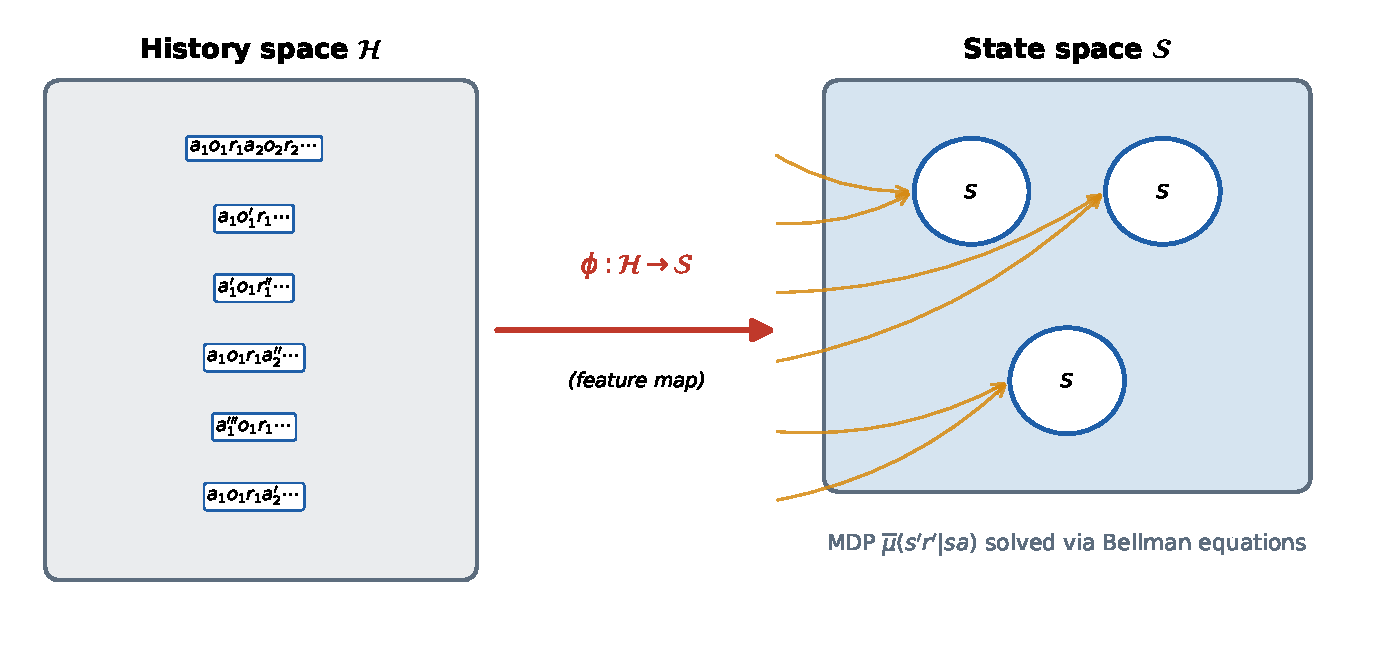
\includegraphics[width=0.48\linewidth]{phi_map_schematic}
\end{frame}

%% ══════════════════════════════════════════════════════════════════════════
\section{14.1 Feature Reinforcement Learning Setup}

\begin{frame}{Feature Maps: From Histories to States}
  \begin{block}{The Feature Map $\phi$}
    A \textbf{feature map} is a function
    \[
      \phi:\Hc\to\Sc, \qquad \Hc:=(\Ec\times\Ac)^*\times\Ec
    \]
    which maps a history space $\Hc$ to a state space $\Sc$, turning our
    problem from a general reinforcement problem into a \textbf{Markov
    decision process (MDP)} over the state space $\Sc$.
  \end{block}
  \textbf{Plain English.} $\Ec=\Oc\times\Rc$ (\textit{observation space}
  $\times$ \textit{reward space}) is the \textbf{percept space} -- what the
  agent perceives at each step -- and $\Ac$ is the \textbf{action space}.
  So $\Hc$ is the set of all finite sequences of actions and percepts. The
  map $\phi$ throws away everything about a history except which
  \textbf{state} $s\in\Sc$ it belongs to. Unless stated otherwise, $\Sc$ is
  assumed finite, and ideally small (in some sense we make precise later).

  \vspace{0.4em}
  \textbf{Notation convention.} In this chapter, $\pi$ (pi) and $\mu$ (mu)
  denote the \textbf{policy} and \textbf{environment} in the original
  general reinforcement learning setting, while $\overline{\pi}$ and
  $\overline{\mu}$ (``pi-bar'', ``mu-bar'') denote the policy and
  environment of the \textbf{derived MDP} setting.
\end{frame}

\begin{frame}{History-Based (Q-)Values}
  The goal of FRL is to use solutions found in the simplified MDP/state
  space setting to build agents with good behavior in the \emph{original}
  general reinforcement learning setting. We already know what ``good
  behavior'' means there: maximizing the discounted expected future reward
  sum, i.e.\ the \textbf{value} (Definition 6.6.1) and \textbf{Q-value}
  (Definition 6.7.1). In this chapter we use \emph{unnormalized}
  infinite-horizon (Q-)Values with geometric discounting in the true
  environment $\mu$:
  \begin{block}{(Q-)Value Functions in the General Setting}
    \[
      V_\mu^\pi(\hlt) := \E^\pi_\mu\!\left[\sum_{k=t}^\infty \gamma^{k-t} r_k \,\middle|\, \hlt\right]
      = \sum_{a_t}\pi(a_t|\hlt)\,Q_\nu^\pi(\hlt,a_t)
    \]
    \[
      Q_\mu^\pi(\hlt,a_t) := \E^\pi_\mu\!\left[\sum_{k=t}^\infty \gamma^{k-t} r_k \,\middle|\, \hlt a_t\right]
      = \sum_{e_t}\nu(e_t|\hlt a_t)\big[r_t+\gamma V_\mu^\pi(h_{1:t})\big]
    \]
  \end{block}
  \textbf{Plain English.} $\gamma$ (gamma) is the \textbf{discount factor}
  (a number in $(0,1)$ making distant rewards count less); $r_k$ is the
  reward at time $k$; $\E^\pi_\mu[\cdot|\hlt]$ is the expectation under
  policy $\pi$ in $\mu$, given history $\hlt$. $V^\pi_\mu(\hlt)$ is the
  value of following $\pi$ from now on; $Q^\pi_\mu(\hlt,a_t)$ is the value
  of taking $a_t$ now, then following $\pi$. The optimal policy is
  $\pi_\mu^*\in\arg\max_\pi V_\mu^\pi(\epsilon)$.
\end{frame}

\begin{frame}{Markov Decision Processes, Recalled}
  \begin{block}{Markov Environment}
    An environment $\overline{\mu}$ is a \textbf{Markov Decision Process
    (MDP)} if it depends only on the most recent observation and action.
    If the environment is Markov, we call the observations \textbf{states}
    (notation $s$, set $\Sc$), and require for all histories $\hlt$, states
    $s_t$, and rewards $r_t$:
    \[
      \overline{\mu}(s_tr_t|\hlt) \;=\; \overline{\mu}(s_tr_t|s_{t-1}a_{t-1})
    \]
  \end{block}
  \textbf{Plain English.} This says the probability of the next
  state/reward pair depends \emph{only} on the immediately preceding state
  and action -- not on how we got there. If the state is fully observed
  ($o_t=s_t$, as in Chapter 11), this is the classical
  \textbf{completely observable MDP} setting. Here, though, the state
  space $\Sc$ for $\overline{\mu}$ is kept separate from the observation
  space $\Oc$ for $\mu$: we abuse notation slightly and write
  $\overline{\mu}:\Sc\times\Ac\to\Delta(\Sc\times\Rc)$ ($\Delta$ denotes
  ``probability distribution over''). We use $\overline{\pi}$ for a
  \textbf{deterministic} Markov policy, which depends only on the previous
  state.
\end{frame}

\begin{frame}{Bellman (Optimality) Equations}
  Because the MDP $\overline{\mu}$ and policy $\overline{\pi}$ depend only
  on the state (and are time-invariant), it is convenient to introduce the
  shorthand $s=s_{t-1}$, $a=a_t$, $s'=s_t$, $r'=r_t$.
  \begin{block}{Bellman Equations (Theorem 6.7.2, specialized to MDPs) -- Eq.\ (14.1.1)}
    \[
      Q_{\overline{\mu}}^{\overline{\pi}}(s,a) = \sum_{s',r'\in\Sc\times\Rc}\overline{\mu}(s'r'|sa)\big[r'+\gamma V_{\overline{\mu}}^{\overline{\pi}}(s')\big],
      \qquad
      V_{\overline{\mu}}^{\overline{\pi}}(s) = Q_{\overline{\mu}}^{\overline{\pi}}(s,\overline{\pi}(s))
    \]
  \end{block}
  \begin{block}{Bellman Optimality Equations -- Eq.\ (14.1.2)}
    \[
      Q_{\overline{\mu}}^*(s,a) = \sum_{s',r'}\overline{\mu}(s'r'|sa)\big[r'+\gamma V_{\overline{\mu}}^*(s')\big],
      \quad
      V_{\overline{\mu}}^*(s) = \max_a Q_{\overline{\mu}}^*(s,a),
      \quad
      \overline{\pi}^*(s)\in\arg\max_a Q_{\overline{\mu}}^*(s,a)
    \]
  \end{block}
  \textbf{Plain English.} The value of a state equals the reward you get
  plus the (discounted) value of wherever you land next, averaged over all
  possible next state/reward pairs $(s',r')$ weighted by their probability
  $\overline{\mu}(s'r'|sa)$. The \textbf{optimal} policy $\overline{\pi}^*$
  simply always picks the action $a$ with the highest $Q^*_{\overline\mu}$
  at the current state. These equations only hold for
  \emph{deterministic} $\overline\pi$, but since we care about optimal
  policies -- which can always be chosen deterministic (Definition
  6.6.1) -- this is not a real restriction.
\end{frame}

\begin{frame}[fragile]{Python: Bellman Equations on a Toy 2-State MDP}
  We solve the Bellman optimality equations (14.1.2) by value iteration on
  a hand-built 2-state MDP $\Sc=\{0,1\}$, $\Ac=\{\text{stay},\text{go}\}$,
  with $\gamma=0.9$.
  \begin{lstlisting}[style=pycode]
gamma = 0.9
S, A = [0, 1], ["stay", "go"]
P = {0: {"stay": {0: .8, 1: .2}, "go": {0: .3, 1: .7}},
     1: {"stay": {0: .1, 1: .9}, "go": {0: .6, 1: .4}}}
R = {0: {"stay": 1.0, "go": 0.0}, 1: {"stay": 2.0, "go": 5.0}}

V = {0: 0.0, 1: 0.0}
for it in range(2000):
    newV = {s: max(R[s][a] + gamma * sum(P[s][a][sp] * V[sp] for sp in S)
                    for a in A) for s in S}
    if max(abs(newV[s] - V[s]) for s in S) < 1e-10:
        V = newV; break
    V = newV
Q = {s: {a: R[s][a] + gamma * sum(P[s][a][sp] * V[sp] for sp in S)
         for a in A} for s in S}
pi = {s: max(A, key=lambda a: Q[s][a]) for s in S}

# Output: converged after 229 iterations
#   V*(0)=24.8031  V*(1)=28.7402;  Q*(0,go)=24.8031  Q*(1,go)=28.7402
#   pi*(0) = go   pi*(1) = go
  \end{lstlisting}
  $V^*$ is the fixed point of taking the best action's $Q^*$ in every state.
\end{frame}

%% ══════════════════════════════════════════════════════════════════════════
\section{14.2 History Aggregation beyond MDPs}

\begin{frame}{Extreme State Aggregation: The Idea}
  \textbf{Extreme state aggregation} [Hut16] is the idea of aggregating
  histories which have \emph{close} (Q-)Values. ``Aggregation'' means a
  many-to-one mapping from histories to states. If we can map (aggregate)
  histories with close (Q-)Values to the same state, then solving this new
  \emph{state} problem should give a good solution to the original
  problem.

  \vspace{0.4em}
  This is in contrast to many other aggregation methods, which try to map
  similar histories to states based on the \emph{contents} of the
  histories (e.g., histories with the same most recent observation get the
  same state). Most remarkably, we do \emph{not} even need to require that
  the history process $\mu$ maps (even approximately) to an MDP -- we will
  instead build a \textbf{surrogate} $\overline\mu$ that behaves as if it
  were one.

  \vspace{0.4em}
  This section shows how such aggregation can lead to well-performing
  agents, and concludes with an explicit construction of a $\phi$ that
  aggregates this way (\textbf{extreme state aggregation}, Section
  14.2.3).
\end{frame}

\subsection{14.2.1 Surrogate MDP and Dispersion Probability}

\begin{frame}{Definition 14.2.1: The Feature Environment}
  Given an observation space $\Oc$, action space $\Ac$, reward space
  $\Rc$, environment $\mu$, state space $\Sc$, and feature map
  $\phi:\Hc\to\Sc$, we construct a \textbf{feature environment}
  $\mu_\phi$. Let $h\in\Hc$ be a history of \emph{any} length (unlike
  $\hlt$, which has length $t$); if $h$ has length $t$, then
  $h'=hao'r'$ is its extension to length $t{+}1$.
  \begin{block}{Definition 14.2.1 (Feature Environment $\mu_\phi$)}
    \[
      \mu_\phi(s'r'|ha) \;:=\; \sum_{o':\phi(hao'r')=s'} \mu(o'r'|ha)
    \]
  \end{block}
  \textbf{Plain English.} $\mu_\phi$ answers: ``given the true environment
  $\mu$, what is the probability of landing in state $s'$ (and getting
  reward $r'$), after taking action $a$?'' We compute it by summing the
  true probability $\mu(o'r'|ha)$ over every observation $o'$ that, once
  appended to the history and mapped through $\phi$, would land us in
  $s'$.

  \vspace{0.4em}
  We have a simple condition for when $\mu_\phi$ happens to already be an
  MDP: this holds if there is an MDP kernel $p:\Sc\times\Ac\to\Delta(\Sc\times\Rc)$
  such that $\mu_\phi(s'r'|ha)=p(s'r'|sa)$ whenever $\phi(h)=s$. The key
  difference to most other state-aggregation methods is that we will
  \emph{not} require $\mu_\phi$ to be an MDP (not even approximately).
\end{frame}

\begin{frame}{Definition 14.2.2: Dispersion Probability}
  Instead we construct a surrogate MDP using a kind of stochastic
  \emph{inverse} of $\phi$.
  \begin{block}{Definition 14.2.2 (Dispersion Probability $B$)}
    Let $B:\Sc\times\Ac\to\Delta(\Hc)$ be a probability distribution on
    histories for each state-action pair, such that $B(h|sa)=0$ if
    $s\neq\phi(h)$. The formal constraints are
    \[
      B(h|sa)\ge 0 \qquad\text{and}\qquad \sum_{h\in\Hc} B(h|sa) = \sum_{h:\phi(h)=s} B(h|sa) = 1 \quad \forall s,a
    \]
  \end{block}
  \textbf{Plain English.} $B$ may be viewed as a stochastic ``inverse'' to
  $\phi$: it assigns non-zero probability \emph{only} to histories $h$ that
  $\phi$ maps to $s$ (i.e.\ $h\in\phi^{-1}(s)$), and for each state-action
  pair those probabilities sum to $1$. Intuitively, $B(h|sa)$ says ``if I
  am told the current state is $s$ and I took action $a$, how likely is it
  that the actual underlying history was $h$?''

  \vspace{0.4em}
  Crucially, the sum defining $B$ ranges over histories of \emph{all}
  lengths, making $B$ a discrete probability over the countable space
  $\Hc$ -- unlike the ``continuous'' probability measure $\mu(h):=\mu(\Gamma_h)$
  over infinite histories defined via cylinder sets $\Gamma_h$.
\end{frame}

\begin{frame}{Definition 14.2.3: The Surrogate MDP}
  \begin{block}{Definition 14.2.3 (Surrogate MDP)}
    Given feature environment $\mu_\phi$ and dispersion probability $B$, we
    define the \textbf{surrogate MDP}:
    \[
      \overline{\mu}(s'r'|sa) \;:=\; \sum_{h\in\Hc} \mu_\phi(s'r'|ha)\,B(h|sa)
    \]
  \end{block}
  \textbf{Plain English.} To predict the next state/reward from $(s,a)$
  under the surrogate MDP, we average the feature environment's prediction
  $\mu_\phi(s'r'|ha)$ over all histories $h$ that could be ``hiding
  behind'' state $s$, weighted by how likely $B$ thinks each one is.

  \begin{block}{Remark 14.2.4 (If $\mu_\phi$ is an MDP, then $\overline\mu=\mu_\phi$)}
    The surrogate-MDP notion is consistent: if $\mu_\phi$ is already an
    MDP, then $\overline\mu=\mu_\phi$ for \emph{any} choice of dispersion
    probability $B$, since
    \[
      \overline{\mu}(s'r'|sa) \equiv \sum_{h:\phi(h)=s}\mu_\phi(s'r'|ha)B(h|sa)
      = \mu_\phi(s'r'|sa)\sum_{h:\phi(h)=s}B(h|sa) = \mu_\phi(s'r'|sa)
    \]
    where the second equality holds iff $\mu_\phi$ is an MDP -- an
    assumption we will \emph{not} make in general.
  \end{block}
\end{frame}

\begin{frame}[allowframebreaks]{Lemma 14.2.5: Dispersion Probability Equivalence}
  \begin{block}{Lemma 14.2.5 (Dispersion Probability Equivalence)}
    For any function $f:\Sc\times\Rc\to\R$, any feature map $\phi$,
    feature function $\mu_\phi$ (Definition 14.2.1), surrogate MDP
    $\overline\mu$ (Definition 14.2.3), with $s':=\phi(h')$ and
    $h'=hao'r'$, it holds
    \[
      \sum_{h\in\Hc}B(h|sa)\sum_{o',r'}\mu(o'r'|ha)f(s',r') \;=\; \sum_{s',r'}\overline{\mu}(s'r'|sa)f(s',r')
    \]
  \end{block}
  \textbf{Plain English.} This says that averaging any function $f$ of the
  \emph{true} next state/reward over $B$ and $\mu$ gives exactly the same
  answer as averaging $f$ directly over the surrogate MDP $\overline\mu$.
  In other words, $\overline\mu$ is a faithful summary of $\mu$, for the
  purposes of computing expectations, once we condition on $s,a$ via $B$.

  \framebreak

  \textbf{Proof.}
  \begin{align*}
    &\sum_{h\in\Hc}B(h|sa)\sum_{o',r'}\mu(o'r'|ha)f(s',r') \\
    &\overset{(a)}{=} \sum_{h\in\Hc}B(h|sa)\sum_{s',r'}\sum_{o':\phi(h')=s'}\mu(o'r'|ha)f(s',r') \\
    &\overset{(b)}{=} \sum_{h\in\Hc}B(h|sa)\sum_{s',r'}\mu_\phi(s'r'|ha)f(s',r') \\
    &\overset{(c)}{=} \sum_{s',r'}\overline{\mu}(s'r'|sa)f(s',r')
  \end{align*}
  For (a) we sum over all $o'$ by first summing over all $o'$ such that
  $\phi(hao'r')=s'$, then summing over all $s'$. In (b) we used Definition
  14.2.1. In (c) we used Definition 14.2.3. $\blacksquare$

  \vspace{0.4em}
  Additionally, with the dispersion probability $B$ we define the
  \textbf{$B$-average} of a Q-value for all histories $\tilde h$ that
  $\phi$ maps to the same state as $h$:
  \[
    \langle Q(h,a)\rangle_B := \sum_{\tilde h\in\Hc} B(\tilde h|\phi(h)a)\,Q(\tilde h,a) \qquad\text{where } s=\phi(h) \tag{14.2.6}
  \]
\end{frame}

\begin{frame}[allowframebreaks]{Lemma 14.2.7: $B$-Average Bounds}
  \begin{block}{Lemma 14.2.7 ($B$-Average Bounds)}
    For any $\mu,\phi,B,\pi,\overline\pi$, define $\overline\mu$ via
    Definitions 14.2.1 and 14.2.3. Then
    \begin{align*}
      \text{If}\quad &|V_\mu^\pi(h)-V_{\overline\mu}^{\overline\pi}(s)|\le\delta \;\;\forall s=\phi(h)
      &&\text{then}\quad |\langle Q_\mu^\pi(h,a)\rangle_B - Q_{\overline\mu}^{\overline\pi}(s,a)| \le \gamma\delta \;\;\forall s=\phi(h),a\\
      \text{If}\quad &|V_\mu^*(h)-V_{\overline\mu}^*(s)|\le\delta \;\;\forall s=\phi(h)
      &&\text{then}\quad |\langle Q_\mu^*(h,a)\rangle_B - Q_{\overline\mu}^*(s,a)| \le \gamma\delta \;\;\forall s=\phi(h),a
    \end{align*}
  \end{block}
  \textbf{Plain English.} If the true value function $V^\pi_\mu$ (on
  histories) and the surrogate value function $V^{\overline\pi}_{\overline\mu}$
  (on states) are close for all histories mapping to a given state, then
  their corresponding \emph{$B$-averaged} Q-values are close too, up to an
  extra factor of $\gamma$ (which only shrinks the gap, since $\gamma<1$).
  The same holds for the optimal (starred) value/Q-functions.

  \framebreak

  \textbf{Proof.} Let $s:=\phi(h)$, $s':=\phi(h')$, $h'=hao'r'$.
  \begin{align*}
    \langle Q_\mu^\pi(h,a)\rangle_B
      &\overset{(a)}{=} \sum_{\tilde h\in\Hc}B(\tilde h|\phi(h)a)Q_\mu^\pi(\tilde h,a) \\
      &\overset{(b)}{=} \sum_{\tilde h\in\Hc}B(\tilde h|\phi(h)a)\sum_{o',r'}\mu(o'r'|\tilde ha)(r'+\gamma V_\mu^\pi(\tilde h')) \\
      &\overset{(c)}{\lessgtr} \sum_{\tilde h\in\Hc}B(\tilde h|\phi(h)a)\sum_{o',r'}\mu(o'r'|\tilde ha)\big(r'+\gamma(V_{\overline\mu}^{\overline\pi}(s')\pm\delta)\big) \\
      &\overset{(d)}{=} \sum_{s',r'}\overline\mu(s'r'|sa)(r'+\gamma V_{\overline\mu}^{\overline\pi}(s')) + \gamma\delta \\
      &\overset{(e)}{=} Q_{\overline\mu}^{\overline\pi}(s,a) \pm \gamma\delta
  \end{align*}
  (a) is (14.2.6). (b) is the Bellman equation for Q-values. (c) is from
  the lemma's assumptions ($c\lessgtr a\pm b$ means $c\le a+b$ and
  $c\ge a-b$). (d) comes from Lemma 14.2.5. (e) is from (14.1.1). Lower and
  upper bounds together give
  $|\langle Q_\mu^\pi(h,a)\rangle_B - Q_{\overline\mu}^{\overline\pi}(s,a)|\le\gamma\delta$.
  The second result follows by replacing $\pi$ with $\pi^*_\mu$ and
  $\overline\pi$ with $\overline\pi^*_{\overline\mu}$; note that in
  general $\pi^*_\mu\neq\overline\pi^*_{\overline\mu}$. $\blacksquare$
\end{frame}

\subsection{14.2.2 (Q-)Value Inheritance for Fixed and Optimal Policy}

\begin{frame}{Theorem 14.2.8: Q-Value Inheritance}
  \begin{block}{Theorem 14.2.8 (Q-Value Inheritance [Hut16, Thm.5])}
    For any $\mu,\phi,B$, define $\overline\mu$ via Definitions 14.2.1 and
    14.2.3. Let $\pi$ be a policy such that
    $|Q_\mu^\pi(h,a)-Q_\mu^\pi(\tilde h,a)|\le\varepsilon_q$ and either
    $\pi(h)=\pi(\tilde h)$ with $\varepsilon_v=0$, or
    $|V_\mu^\pi(h)-V_\mu^\pi(\tilde h)|\le\varepsilon_v$, for all
    $\phi(h)=\phi(\tilde h)$ and all $a$. Then for all $a$ and $h$:
    \[
      |Q_\mu^\pi(h,a)-Q_{\overline\mu}^{\overline\pi}(s,a)| \le \frac{\varepsilon}{1-\gamma}
      \qquad\text{and}\qquad
      |V_\mu^\pi(h)-V_{\overline\mu}^{\overline\pi}(s)| \le \frac{\varepsilon}{1-\gamma}
    \]
    where $\overline\pi(s)=\pi(h)$, $s=\phi(h)$, and $\varepsilon=\varepsilon_q+\varepsilon_v$.
  \end{block}
  \textbf{Plain English.} If two histories $h,\tilde h$ map to the same
  state and have close Q-values (within $\varepsilon_q$) and either the
  \emph{same} action under $\pi$ or close values (within $\varepsilon_v$),
  then the true Q-value/value on histories is close to the surrogate MDP's
  Q-value/value on states -- within $\varepsilon/(1-\gamma)$. So being
  careful to aggregate histories with similar behavior is enough to
  ``inherit'' good performance from the small MDP.
\end{frame}

\begin{frame}[allowframebreaks]{Proof of Theorem 14.2.8}
  \textbf{Proof.} Let
  \[
    \delta := \sup_{s=\phi(h),a}\big|Q_\mu^\pi(h,a)-Q_{\overline\mu}^{\overline\pi}(s,a)\big| \tag{14.2.9}
  \]
  \textbf{Step 1.} We show $|V_\mu^\pi(h)-V_{\overline\mu}^{\overline\pi}(s)|\le\delta+\varepsilon_v\;\forall s=\phi(h)$
  (Eq.\ 14.2.10). Under either condition of the theorem this follows from
  (6.7.4) and (14.1.1) and the definition of the supremum. For the
  or-condition, let $\overline\pi(s):=\pi(\tilde h)$ for some
  $\tilde h\in\phi^{-1}(s)$. Then
  \[
    |V_\mu^\pi(h)-V_{\overline\mu}^{\overline\pi}(s)|
    \overset{(a)}{\le} |V_\mu^\pi(\tilde h)-V_{\overline\mu}^{\overline\pi}(s)|+\varepsilon_v
    \overset{(b)}{=} |Q_\mu^\pi(\tilde h,\tilde a)-Q_{\overline\mu}^{\overline\pi}(s,\tilde a)|+\varepsilon_v
    \overset{(c)}{\le} \delta+\varepsilon_v
  \]
  where (a) is the assumptions plus the triangle inequality, (b) uses
  (6.7.4) and (14.1.1) with $\tilde a=\overline\pi(s)=\pi(\tilde h)$, and
  (c) is the definition of $\delta$.

  \framebreak

  \textbf{Step 2.} By Lemma 14.2.7, (14.2.10) implies
  \[
    |\langle Q_\mu^\pi(h,a)\rangle_B - Q_{\overline\mu}^{\overline\pi}(s,a)| \le \gamma(\delta+\varepsilon_v) \quad\forall s=\phi(h) \tag{14.2.11}
  \]
  By the assumption on $Q^\pi_\mu$ and $B$, for $s=\phi(h)$ we have (using
  $c\lessgtr a\pm b$ notation again)
  \[
    \langle Q_\mu^\pi(h,a)\rangle_B = \sum_{\tilde h:\phi(\tilde h)=s} B(\tilde h|ha)Q_\mu^\pi(\tilde h,a)
    \lessgtr \sum_{\tilde h:\phi(\tilde h)=s} B(\tilde h|ha)(Q_\mu^\pi(h,a)\pm\varepsilon_q)
    = Q_\mu^\pi(h,a)\pm\varepsilon_q
  \]
  Together with (14.2.11) this implies
  $|Q_\mu^\pi(h,a)-Q_{\overline\mu}^{\overline\pi}(s,a)|\le\gamma(\delta+\varepsilon_v)+\varepsilon_q$,
  hence $\delta\le\gamma(\delta+\varepsilon_v)+\varepsilon_q$, and
  rearranging gives $\delta\le\frac{\varepsilon_q+\gamma\varepsilon_v}{1-\gamma}$.
  Inserting this bound into (14.2.9) and (14.2.10) gives the bounds in the
  theorem. $\blacksquare$
\end{frame}

\begin{frame}{Theorem 14.2.12: Value Inheritance}
  \begin{block}{Theorem 14.2.12 (Value Inheritance [Hut16, Thm.6])}
    For any $\mu,\phi,B$, define $\overline\mu$ via Definitions 14.2.1 and
    14.2.3. Let $\pi$ be a policy such that
    $|V_\mu^\pi(h)-V_\mu^\pi(\tilde h)|\le\varepsilon$ for all
    $\phi(h)=\phi(\tilde h)$. Then for all $a$ and $h$:
    \[
      |V_\mu^\pi(h)-V_{\overline\mu}^{\overline\pi}(s)| \le \frac{\varepsilon}{1-\gamma}
      \qquad\text{and}\qquad
      |Q_{\overline\mu}^{\overline\pi}(s,a)-\langle Q_\mu^\pi(h,a)\rangle_B| \le \frac{\varepsilon\gamma}{1-\gamma}
    \]
    where $\overline\pi(s)=\pi(h)$ and $s=\phi(h)$.
  \end{block}
  \textbf{Plain English.} A companion result to Theorem 14.2.8: this time
  we only need the \emph{value} function (not Q-values) to be close on
  aggregated histories, and we get a similar guarantee -- the ``closeness''
  of aggregated states is inherited by the MDP's value function
  $V_{\overline\mu}^{\overline\pi}$.
\end{frame}

\begin{frame}{Example 14.2.13: Aggregation to a Non-MDP}
  Consider a process $\mu$ that is itself an MDP in the observations, with
  transition matrix $T$ and reward function $R$, i.e.\
  $\mu(o'r'|ha)=T^a_{oo'}R^{ar'}_{oo'}$, where $o$ is the last observation
  in $h$. Concretely, with observation space $\Oc=\{00,01,10,11\}$:
  \[
    T = \begin{pmatrix}\cdot&\tfrac12&\tfrac12&\cdot\\ \tfrac12&\cdot&\cdot&\tfrac12\\ \cdot&1&\cdot&\cdot\\ 1&\cdot&\cdot&\cdot\end{pmatrix},
    \qquad
    R = \begin{pmatrix}\gamma/2/(1+\gamma)\\ (1+\gamma/2)/(1+\gamma)\\ 0\\ 1\end{pmatrix}
  \]
  This is an action-independent Markov process with a deterministic reward
  $R$ (i.e.\ $\mu(o'r'|ha)=T_{oo'}\cdot[\![r'=R(o)]\!]$, with $[\![\cdot]\!]$
  the indicator function).
\end{frame}

\begin{frame}{Example 14.2.13, Pictured}
  \centering
  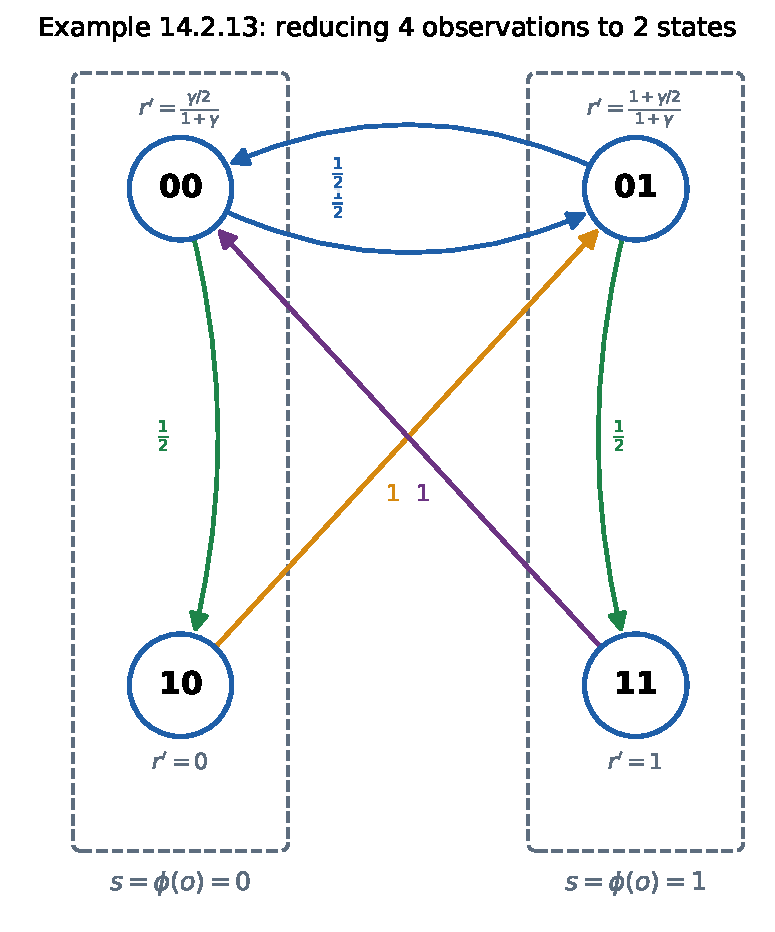
\includegraphics[width=0.32\linewidth]{example_4state_diagram}

  \raggedright
  \vspace{0.2em}
  Each circle is a raw observation $o\in\{00,01,10,11\}$; arrows show
  transition probabilities from $T$; $r'$ labels show the deterministic
  reward $R(o)$ for leaving that observation. Dashed boxes show the
  2-state aggregation we consider next.
\end{frame}

\begin{frame}{Example 14.2.13, Continued: The Reduction Is Not Markov}
  Consider the reduction
  \[
    s_t := \phi(h_t) := \begin{cases}0 & \text{if } o_t=00\text{ or }10\\ 1 & \text{if } o_t=01\text{ or }11\end{cases}
    \;\in\; \Sc:=\{0,1\}
  \]
  The reduced process $\mu_\phi$ is \textbf{not} (even approximately)
  Markov:
  \[
    \mu_\phi(s'=0|o=00) = T_{00,00}+T_{00,10} = 0+\tfrac12 = \tfrac12
    \;\neq\;
    \mu_\phi(s'=0|o=10) = T_{10,00}+T_{10,10} = 0+0 = 0
  \]
  \textbf{Plain English.} Being told only ``$s=0$'' is not enough to
  predict the next state: it matters whether the underlying observation
  was $00$ or $10$, and those give \emph{different} next-state
  probabilities. So $\mu$ violates the \textbf{bisimulation condition}
  [GDG03], and raw observations $00,10$ have a large ``bisimulation
  distance'' [FPP04,Ort07].

  \vspace{0.4em}
  \textbf{Yet the (Q-)Values agree.} One can verify directly that
  $V(o_t):=V^\pi(h_t)=Q^\pi(h_t,a_t)\;\forall a_t$ satisfies
  \[
    V(00)=V(10)=\frac{\gamma}{1-\gamma^2} \qquad\text{and}\qquad V(01)=V(11)=\frac{1}{1-\gamma^2}
  \]
  That is, $V$ and $Q$ are \textbf{$\phi$-uniform}: they agree exactly on
  histories $\phi$ maps together. The conditions of Theorems 14.2.8 and
  14.2.12 hold exactly ($\varepsilon=0$), so all four raw observations can
  be aggregated into just \textbf{two} states, \emph{despite}
  $\mu_\phi\notin$ MDP (the policy is irrelevant here and can be chosen
  constant). $\blacklozenge$
\end{frame}

\begin{frame}[fragile]{Python: Reproducing Example 14.2.13}
  We rebuild $T$ and $R$ exactly, verify $\mu_\phi(s'=0|o)$ against the
  book's values, then solve $V(o)=R(o)+\gamma\sum_{o'}T_{oo'}V(o')$
  directly (recall $R(o)$ attaches to the \emph{current} observation, per
  $\mu(o'r'|ha)=T_{oo'}\cdot[\![r'=R(o)]\!]$) and compare to the closed
  forms.
  \begin{lstlisting}[style=pycode]
import numpy as np
gamma = 0.9
obs = ["00", "01", "10", "11"]
T = np.array([[0, .5, .5, 0], [.5, 0, 0, .5],
              [0, 1, 0, 0],  [1, 0, 0, 0]])
Rvec = np.array([(gamma/2)/(1+gamma), (1+gamma/2)/(1+gamma), 0.0, 1.0])
phi = lambda o: 0 if o in ("00", "10") else 1

for i, o in enumerate(obs):
    p0 = sum(T[i, obs.index(op)] for op in obs if phi(op) == 0)
    print(f"mu_phi(s'=0|o={o}) = {p0}")

Vsol = np.linalg.solve(np.eye(4) - gamma * T, Rvec)   # V = R + gamma*T@V

# Output:
# mu_phi(s'=0|o=00) = 0.5   mu_phi(s'=0|o=01) = 0.5
# mu_phi(s'=0|o=10) = 0.0   mu_phi(s'=0|o=11) = 1.0
# solved V(00)=4.736842  V(01)=5.263158  V(10)=4.736842  V(11)=5.263158
# matches gamma/(1-gamma^2)=4.736842 and 1/(1-gamma^2)=5.263158 exactly.
  \end{lstlisting}
\end{frame}

\subsection{14.2.3 Extreme State Aggregation}

\begin{frame}{Theorem 14.2.14: Optimal Q-Value Inheritance}
  \begin{block}{Theorem 14.2.14 (Optimal Q-Value Inheritance [Hut16, Thm.8])}
    For any $\mu,\phi,B$, define $\overline\mu$. Assume
    $|Q_\mu^*(h,a)-Q_\mu^*(\tilde h,a)|\le\varepsilon$ for all
    $\phi(h)=\phi(\tilde h)$ and all $a$. Then for all $a$, $h$, and
    $s=\phi(h)$:
    \begin{itemize}
      \item $|Q_\mu^*(h,a)-Q_{\overline\mu}^*(s,a)|\le\frac{\varepsilon}{1-\gamma}$
        and $|V_\mu^*(h)-V_{\overline\mu}^*(s)|\le\frac{\varepsilon}{1-\gamma}$
      \item $0\le Q_\mu^*(h,a)-Q_\mu^{\tilde\pi}(h,a)\le\frac{2\varepsilon\gamma}{(1-\gamma)^2}$
        and $0\le V_\mu^*(h)-V_\mu^{\tilde\pi}(h)\le\frac{2\varepsilon\gamma}{(1-\gamma)^2}$
      \item If $\varepsilon=0$, then $\pi^*(h)=\overline\pi^*_{\overline\mu}(s)$
    \end{itemize}
    where $\tilde\pi(h):=\overline\pi^*_{\overline\mu}(s)$.
  \end{block}
  \textbf{Plain English.} If histories that $\phi$ maps together have
  close \emph{optimal} Q-values, then the optimal Q-values/values of
  $\overline\mu$ (on states) are close to those of $\mu$ (on histories),
  \emph{and} the ``uplifted'' policy $\tilde\pi$ (act according to the
  small MDP's optimal policy) is itself close to optimal in the original
  problem. When $\varepsilon=0$ exactly, the uplifted policy \emph{is} the
  optimal policy.
\end{frame}

\begin{frame}{Why This Theorem Matters, and a Caveat}
  This theorem shows that when $\phi$ aggregates histories with close
  optimal Q-values, we can aggregate histories \emph{as much as we wish},
  as long as the optimal Q-value function and policy remain approximately
  representable as functions of the aggregated states. Whether the reduced
  process $\mu_\phi$ is Markov or not is \textbf{immaterial}. We can use
  the surrogate MDP $\overline\mu$ to find an $\varepsilon$-optimal policy
  for $\mu$ -- this will prove useful when constructing a map $\phi$ that
  satisfies the theorem's assumptions.

  \begin{block}{Remark 14.2.15 (No Optimal Value Inheritance)}
    The Q-value bound generalizes naturally from Theorem 14.2.12 to the
    optimal case, but somewhat surprisingly the \emph{value} bound does
    \textbf{not} generalize to optimal policies [Hut16, Thm.10].
  \end{block}
\end{frame}

\begin{frame}{Definition 14.2.16: Extreme State Aggregation}
  We now give an example of an extreme state aggregation map $\phi$ that
  satisfies the premises of Theorem 14.2.14.
  \begin{block}{Definition 14.2.16 (Extreme State Aggregation)}
    Consider $\phi^{ESA}$ that maps each history to the
    \textbf{vector-over-actions of optimal Q-values} $Q^*_\mu(h,\cdot)$,
    discretized to some finite $\varepsilon$-grid:
    \[
      \phi^{ESA}(h) := \left(\left\lfloor \frac{Q^*_\mu(h,a)}{\varepsilon}\right\rfloor\right)_{a\in\Ac}
      \;\in\; \left\{0,\ldots,\left\lfloor\frac{1}{\varepsilon(1-\gamma)}\right\rfloor\right\}^{\Ac} =: \Sc
    \]
  \end{block}
  \textbf{Plain English.} $\lfloor\cdot\rfloor$ is the \textbf{floor}
  (round-down) function. For \emph{each} action $a$, we take the true
  optimal Q-value $Q^*_\mu(h,a)$, divide it by a small grid spacing
  $\varepsilon$, and round down -- like snapping a real number onto a
  grid. The state is the resulting tuple of grid cells, one entry per
  action. Histories with $\varepsilon$-close $Q^*_\mu$-values in
  \emph{every} action land in exactly the same grid cell, hence the same
  state -- this is obvious from the construction.

  \vspace{0.4em}
  Given $\mu,B,\phi$ we build $\overline\mu$, find its optimal policy
  $\overline\pi^*_{\overline\mu}$, and \emph{uplift} it via
  $\tilde\pi(h):=\overline\pi^*_{\overline\mu}(\phi(h))$. By Theorem
  14.2.14, $\tilde\pi(h)$ is $\varepsilon'$-optimal in $\mu$, where
  $\varepsilon':=2\varepsilon(1-\gamma)^2$ (when $\varepsilon=0$, $Q^*_\mu$
  is bounded by $\frac{1}{1-\gamma}$).
\end{frame}

\begin{frame}[allowframebreaks]{Theorem 14.2.17: Extreme $\phi$ and Its Size Bound}
  \begin{block}{Theorem 14.2.17 (Extreme $\phi$)}
    For every process $\mu$, there exists a feature map $\phi$ (Definition
    14.2.16), namely $\phi^{ESA}$, and an MDP $\overline\mu$ (Definitions
    14.2.1, 14.2.3), whose optimal policy $\overline\pi^*$ is an
    $\varepsilon'$-optimal policy $\tilde\pi(h):=\overline\pi^*(\phi(h))$
    for $\mu$. The size of the MDP $\overline\mu$ is bounded (uniformly
    for any $\mu$) by
    \[
      |\Sc| \;\le\; \left(\frac{3}{\varepsilon'(1-\gamma)^3}\right)^{|\Ac|}
    \]
  \end{block}
  \textbf{Plain English.} No matter how complicated $\mu$ is, there is
  \emph{always} some finite-state MDP -- built purely from the shape of
  $Q^*_\mu$ -- whose optimal policy, once ``uplifted'' back to histories,
  performs within $\varepsilon'$ of optimal. And its size does not depend
  on the observation or reward space at all, only on $\varepsilon'$,
  $\gamma$, and the number of actions $|\Ac|$.

  \framebreak

  \textbf{Proof.} If $\varepsilon'>\frac{1}{1-\gamma}$ then \emph{any}
  policy is $\varepsilon'$-optimal (since $Q_\mu^*\le\frac{1}{1-\gamma}<\varepsilon'$),
  so the result holds trivially by choosing a trivial state class
  $|\Sc|=1$. In the case $\varepsilon'\le\frac{1}{1-\gamma}$, from the
  definition of $\Sc$ in Definition 14.2.16 we have
  \[
    |\Sc| = \left(\left\lfloor\frac{1}{\varepsilon(1-\gamma)}\right\rfloor+1\right)^{|\Ac|}
    = \left(\left\lfloor\frac{2}{\varepsilon'(1-\gamma)^3}\right\rfloor+1\right)^{|\Ac|}
    \le \left(\frac{3}{\varepsilon'(1-\gamma)^3}\right)^{|\Ac|} \qquad\blacksquare
  \]

  \framebreak

  Interestingly, these bounds do \textbf{not} depend on the size of the
  observation space, the reward space, or the complexity of $\mu$ -- because
  extreme state aggregation only cares about aggregating histories with
  similar (Q-)Values, regardless of what the original spaces or the
  resulting Markov property look like.

  \vspace{0.4em}
  Unfortunately the bound is \emph{exponential} in the action space size,
  and due to the high powers of $\varepsilon'$ and $1-\gamma$ can be very
  large. But it was shown in [MH21b,MH21a] that if the action space is
  \emph{sequentialized} into binary actions, the bound improves from
  exponential to \emph{logarithmic} in $|\Ac|$ -- a double-exponential
  improvement:
  \[
    |\Sc| \;\le\; \frac{17(\log|\Ac|)^3}{\varepsilon'(1-\gamma)^3} \tag{14.2.18}
  \]
  \centering
  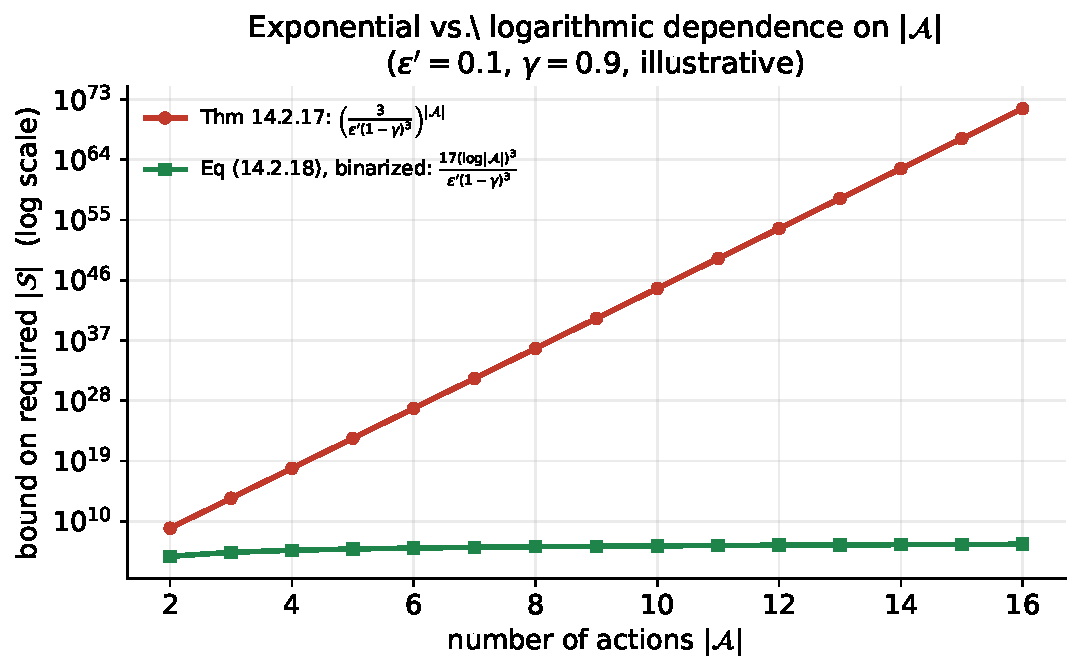
\includegraphics[width=0.62\linewidth]{state_bound_comparison}
\end{frame}

\begin{frame}{Section 14.2.4: Feature Reinforcement Learning in Practice}
  In practice, we do not know $Q^*_\mu$ (which would imply the optimal
  policy is already known), so we do not have access to the extreme
  $\phi$-map of Definition 14.2.16. That map is \emph{not} meant for
  practical use -- it exists to demonstrate that a $\phi$-map satisfying
  our theorems' premises exists at all.

  \vspace{0.4em}
  Reinforcement learning \emph{learns} $Q^*_\mu$ from samples. Taking a
  model-based approach, we can first learn $\overline\mu$, then use
  (14.1.2) to compute $Q^*_{\overline\mu}$. It turns out that for a very
  particular choice of $B$, we can follow \emph{any} convenient behavior
  policy (off-policy learning), and a simple frequency estimate -- counting
  $(s,a,r',s')$-pairs in the reduced history $\overline h$ (see Section
  14.3.1) -- indeed estimates $\overline\mu$, despite being a surrogate MDP
  only related to the true sampling distribution $\mu$ via Definitions
  14.2.1 and 14.2.3.

  \vspace{0.4em}
  \textbf{The chicken-egg problem.} All this still assumed $\phi$ is
  given. Ultimately the goal of FRL is to also \emph{learn} a map $\phi$
  satisfying the premises -- but this again requires first finding
  $Q^*_\mu$, and thus defeats the purpose. This is a classical, but
  solvable, chicken-egg problem: algorithms to learn $\phi$ were proposed
  in [Hut16] and developed in [Maj21].
\end{frame}

%% ══════════════════════════════════════════════════════════════════════════
\section{14.3 Feature MDP}

\begin{frame}{Feature MDP ($\Phi$MDP): A Practical Construction}
  In the previous section we discussed ideal properties for $\phi$
  (aggregating close Q-values), then used that criterion to construct an
  explicit (but impractical) $\phi$. This section provides a
  \textbf{practical} method for iteratively constructing $\phi$, based on
  a \textbf{cost function} over choices of $\phi$ [Hut09f,Das16].

  \vspace{0.4em}
  \textbf{A crucial difference:} here we \emph{require} the aggregation to
  be approximately an MDP. We want $\phi$ to map to a small state space,
  yet large enough that the resulting state dynamics is (still
  approximately) an MDP. So the cost function must balance $\phi$'s with
  small range against $\phi$'s that lead to good (approximate) MDPs, and
  should be minimal for the ``best'' compromise -- an idea in the spirit
  of the \textbf{MDL principle}.
  \begin{center}
    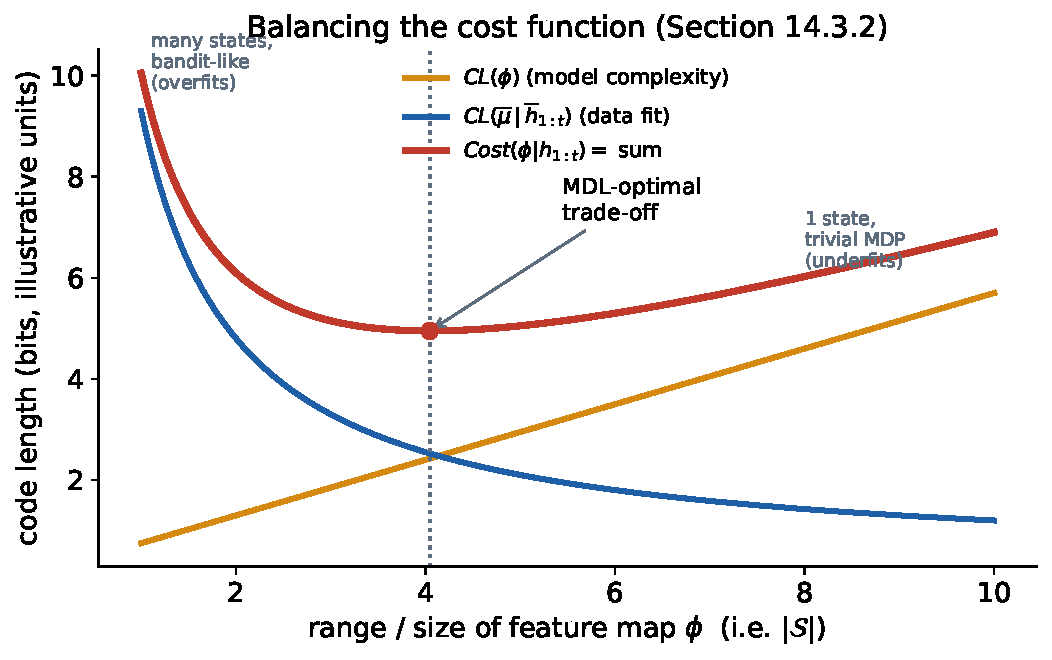
\includegraphics[width=0.42\linewidth]{cost_function_tradeoff}
  \end{center}
\end{frame}

\subsection{14.3.1 Feature Learning}

\begin{frame}{Definition 14.3.1: Feature Map Cost}
  \begin{block}{Definition 14.3.1 (Feature Map Cost)}
    The $\mathit{Cost}$ of $\phi:\Hc\to\Sc$ on $h_{1:t}$ is a measure of
    the quality of the feature map $\phi$ given history $h_{1:t}$.
  \end{block}
  \textbf{Plain English.} We delay the exact choice of $\mathit{Cost}$
  until Section 14.3.2. Ideally $\arg\min_\phi \mathit{Cost}(\phi|h_{1:t})$
  could be computed exactly, but for most interesting/useful choices of
  $\mathit{Cost}$ this is intractable, so we turn to iterative methods
  instead.

  \vspace{0.4em}
  \textbf{Suffix feature maps.} For concreteness, we consider the class of
  feature maps $\{\phi_\Sc\}$ that take the \emph{most recent observations}
  as state: the state space forms a \textbf{suffix set}
  $\Sc\subset\Oc^*$, and $\phi_\Sc(h_{1:t})=o_{k:t}$ for the unique $k$
  such that $o_{k:t}\in\Sc$. (We can generalize to non-binary alphabets or
  binarize $\Oc$ first and assume $\Sc\subset\B^*$.) We write $s_{>1}$ to
  denote $s$ without its first element.
\end{frame}

\begin{frame}{What $\Phi$Improve Does}
  $\Phi$Improve modifies a state space $\Sc$ by either \textbf{splitting}
  one state into several new states, or \textbf{merging} several states
  (if capable of merging) into one -- in suffix-tree jargon, expanding or
  shrinking the suffix tree at some leaf nodes. If the resulting $\phi'$
  has lower $Cost$, the algorithm outputs $\phi'$; otherwise it outputs the
  unchanged $\phi$ (but sometimes accepts a \emph{slightly worse} $\phi'$
  anyway, to escape local minima -- via the $\log(q)$ random-acceptance
  test on the algorithm's last line). The pseudocode is on the next slide.
\end{frame}

\begin{frame}[fragile]{Algorithm 14.1: $\Phi$Improve}
  \begin{algorithmic}[1]
    \Statex \textbf{Input:} State space $\Sc$; feature map $\phi_\Sc:\Hc\to\Sc$; history $\hlt$
    \Statex \textbf{Output:} Improved feature map $\phi_{\Sc'}:\Hc\to\Sc'$
    \State Randomly choose a state $s\in\Sc$
    \State Let $p,q$ be uniform random numbers in $[0,1]$
    \State $\Sc':=\Sc$;\quad $\phi_{\Sc'}:=\phi_\Sc$
    \If{$p>1/2$}
      \State $\Sc' := (\Sc\setminus\{s\})\cup\{os:o\in\Oc\}$ \Comment{Split $\{s\}$ into $\{os:o\in\Oc\}$}
      \State $\phi_{\Sc'}(h)\in\{os:o\in\Oc\}$ for all $h$ s.t. $\phi_\Sc(h)=s$ \Comment{chosen by some rule, e.g.\ randomly}
    \ElsIf{$\{os_{>1}:o\in\Oc\}\subseteq\Sc$}
      \State $\Sc' := (\Sc\setminus\{os_{>1}:o\in\Oc\})\cup\{s_{>1}\}$ \Comment{Merge $\{os_{>1}:o\in\Oc\}$ into $\{s_{>1}\}$}
      \State $\phi_{\Sc'}(h):=s_{>1}$ for all $h$ such that $\phi_\Sc(h)\in\{os_{>1}:o\in\Oc\}$
    \EndIf
    \If{$\mathit{Cost}(\phi_\Sc,\hlt)-\mathit{Cost}(\phi_{\Sc'},\hlt) > \log(q)$}
      \State \textbf{return} $\phi_{\Sc'}$
    \Else
      \State \textbf{return} $\phi_\Sc$
    \EndIf
  \end{algorithmic}
\end{frame}

\begin{frame}{Split and Merge, Pictured}
  \centering
  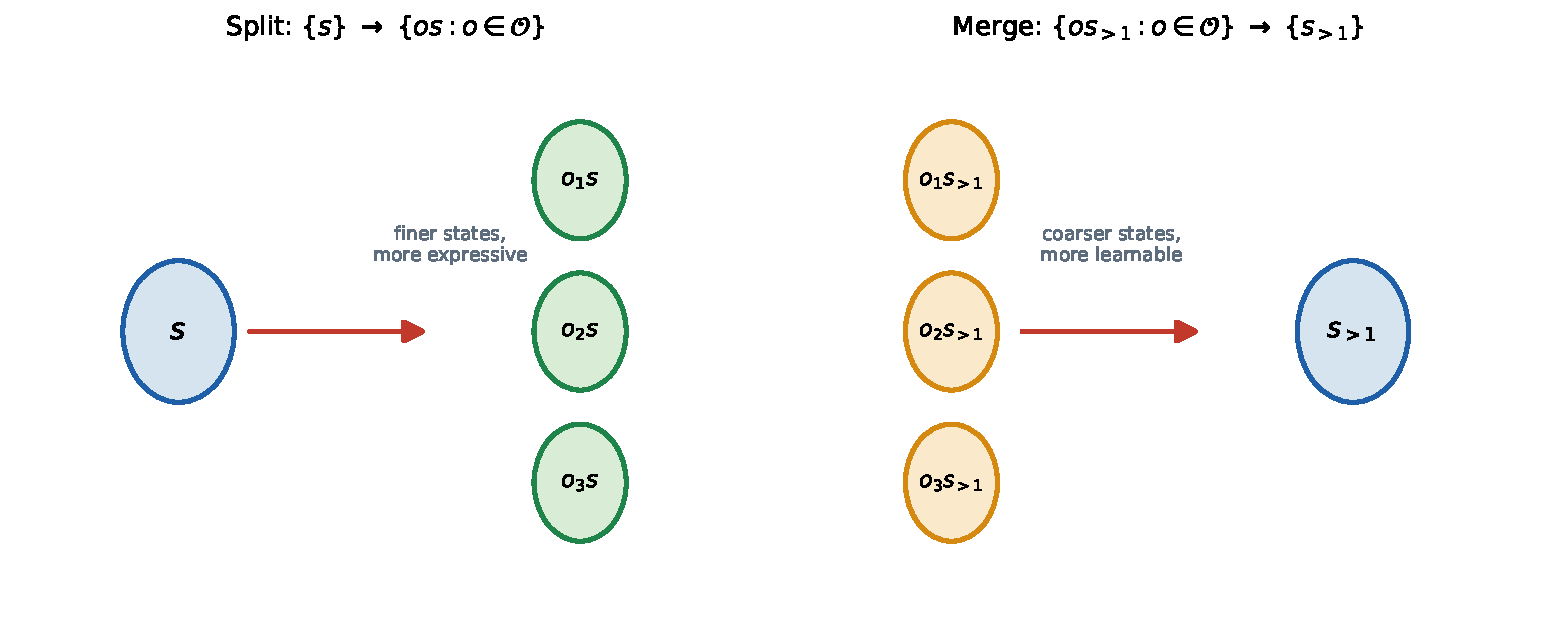
\includegraphics[width=0.92\linewidth]{phi_improve_split_merge}

  \raggedright
  \vspace{0.3em}
  \textbf{Split} increases the resolution of the state space (more, finer
  states) so that the resulting dynamics can capture more structure.
  \textbf{Merge} does the opposite: it coarsens the state space, trading
  some expressiveness for a smaller, more easily learned MDP. $\Phi$Improve
  proposes one such move at random and keeps it only if the total
  $\mathit{Cost}$ improves (or, occasionally, even if it does not -- to
  avoid getting stuck).
\end{frame}

\begin{frame}{Building the MDP: Frequency Estimation}
  Given a feature map $\phi$ we construct the state at each time step as
  $\phi$ of the history, e.g.\ $s_t=\phi(h_{1:t})$. We can then build a
  \textbf{state history} $\overline h_{1:t} := a_1r_1s_1\ldots a_tr_ts_t$.
  Given the state history, we \emph{approximate} the dynamics of the MDP
  through \textbf{frequency estimation} on the transitions of the MDP:
  \begin{block}{Frequency-Estimate MDP -- Eq.\ (14.3.2)}
    \[
      \overline\mu(s'r'|s,a) := \begin{cases}
        \dfrac{N(sar's',\overline h_{1:t})}{N(sa,\overline h_{1:t})} & \text{if } N(sa,\overline h_{1:t})>0\\[4pt]
        0 & \text{otherwise}
      \end{cases}
    \]
  \end{block}
  \textbf{Plain English.} $N(sar's',\overline h_{1:t})$ counts how many
  times the transition $(s,a)\to(s',r')$ has occurred in the state history
  so far, and $N(sa,\overline h_{1:t})$ counts how many times $(s,a)$
  occurred at all. Dividing gives the empirical (observed) probability of
  each transition -- the most natural estimate one could use. (Strictly
  this is only an \emph{estimate} $\hat{\overline\mu}$ of $\overline\mu$.)
\end{frame}

\begin{frame}[fragile]{Algorithm 14.2: The $\Phi$MDP Agent}
  \begin{algorithmic}[1]
    \Statex \textbf{Require:} Action Space $\Ac$; Percept Space $\Ec=\Oc\times\Rc$
    \Statex \textbf{Input:} Percept stream $e_1,e_2,e_3,\ldots$
    \Statex \textbf{Output:} Action stream $a_1,a_2,a_3,\ldots$
    \State $\Sc:=\{\epsilon\}$;\quad $\phi(h):=\epsilon,\;\phi'(h):=\epsilon\;\forall h$;\quad $h_0,\overline h_0,a_0,e_0:=\epsilon$
    \For{$t=1,\ldots$}
      \State $\phi':=\phi$
      \While{waiting for next $e_t$}
        \State $\phi':=\Phi\text{Improve}(\Sc,\phi',\hlt)$
        \If{$\mathit{Cost}(\phi'|\hlt) < \mathit{Cost}(\phi|\hlt)$}
          \State $\phi:=\phi'$
        \EndIf
      \EndWhile
      \State Receive $e_t$ from environment $\mu$
      \State $h_{1:t}:=h_{<t}a_te_t$;\quad $s_t:=\phi(h_{1:t})$;\quad $\overline h_{1:t}:=\overline h_{<t}a_tr_ts_t$;\quad $\Sc:=\Sc\cup\{s_t\}$
      \State Construct $\overline\mu$ by (14.3.2)
      \State $a_t:=\arg\max_a Q^*_{\overline\mu}(s_t,a)$;\quad output action $a_t$
    \EndFor
  \end{algorithmic}
\end{frame}

\begin{frame}{What Algorithm 14.2 Does}
  While waiting for the next percept, the agent keeps proposing improved
  feature maps via $\Phi$Improve and switches to them if they are cheaper.
  Once the percept arrives, it updates its history/state, rebuilds the MDP
  via frequency estimation, and acts greedily according to the resulting
  $Q^*_{\overline\mu}$.
  \vspace{0.2em}
  \centering
  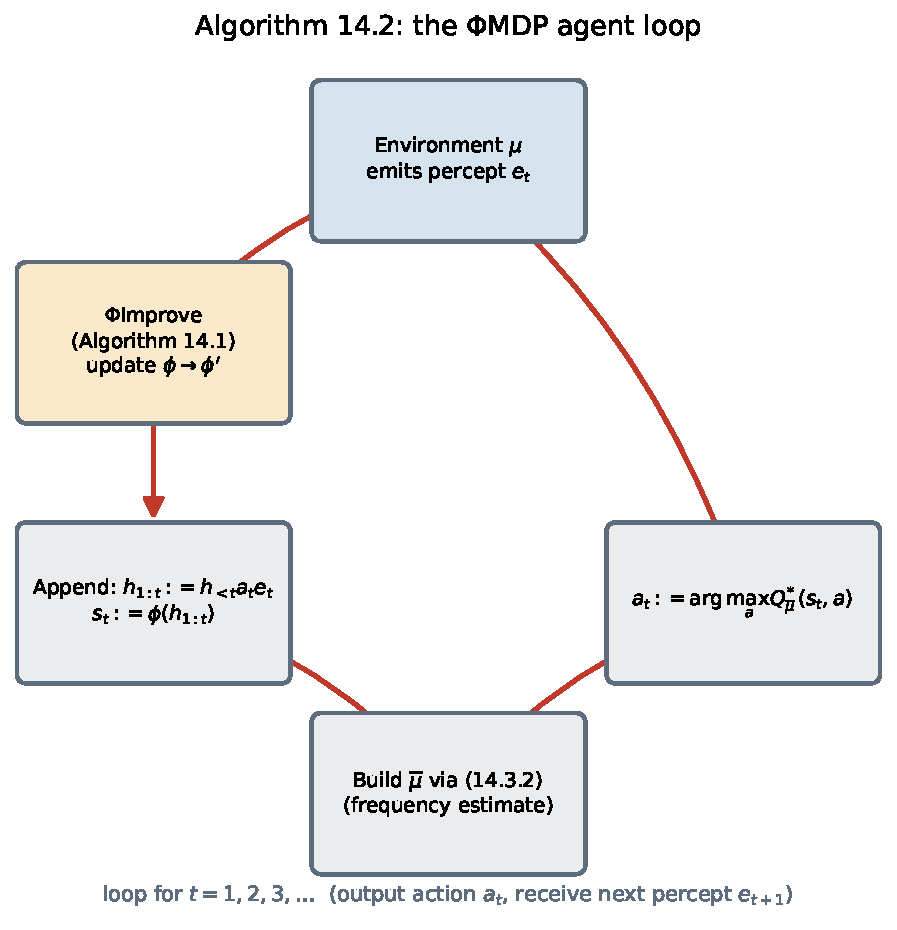
\includegraphics[width=0.4\linewidth]{phimdp_loop_diagram}
\end{frame}

\begin{frame}{A Note on Exploration}
  To ensure sufficient exploration, we can set the reward to be
  \textbf{high} for unexplored state-action interactions when estimating
  $Q^*_{\overline\mu}$ -- an ``optimism'' trick reminiscent of Chapter 9.
  We can solve $Q^*_{\overline\mu}$ efficiently with policy iteration,
  value iteration, or another polynomial-time method. Note that by
  construction, the agent has always \emph{visited} every state, but it
  has not necessarily \emph{taken every action} in every state.

  \vspace{0.4em}
  Using $\Phi$MDP we are able to solve the hard problem of
  general/history-based reinforcement learning by mapping the problem to
  the easier MDP setting, for which we have efficient solutions.
\end{frame}

\subsection{14.3.2 Choices of the Cost Function}

\begin{frame}{Balancing Two Extremes}
  Since we are interested in choices of $\phi$ that let the resulting
  $\Phi$MDP agent perform well, we want $\phi$ to result in states that
  capture the dynamics of the underlying environment $\mu$ sufficiently
  well. Many immediate questions arise, so let's examine two extremes:

  \begin{itemize}
    \item We could choose a $\phi$ that maps every unique history to a
      \emph{different} state. This fully captures the dynamics of $\mu$,
      but we are also interested in \emph{solving} the resulting MDP --
      and with this choice, the resulting MDP is exactly as hard as the
      original problem.
    \item We could instead choose a $\phi$ that maps \emph{all} histories
      to a single state. The resulting MDP (now a bandit problem) has
      many effective algorithmic solutions -- but since it does not
      capture the correct dynamics of $\mu$, it will likely not perform
      well.
  \end{itemize}
  We need a balance between these two extremes. To this end we turn to
  \textbf{simplicity} (as we often do in this book) as a guiding
  principle -- surely both extreme choices of $\phi$ above are simple, if
  we are only interested in \emph{states}. We are interested in using
  \emph{both} the states and rewards of our resulting MDP; however, our
  $\phi$ is only responsible for the states -- the rewards the $\Phi$MDP
  agent is given are the true rewards from the environment $\mu$.
\end{frame}

\begin{frame}{The MDL-Inspired Cost Function}
  We take inspiration from the \textbf{MDL principle} (minimum description
  length) and measure the simplicity of a mapping $\phi$ given a history
  $h_{1:t}$ as the size of an encoding of $h_{1:t}$ with $\phi$, plus the
  size of encoding $\phi$ itself. By ``an encoding of $h_{1:t}$ given
  $\phi$'' we mean an encoding of the resulting $\overline\mu$ given
  $\phi$. Because $\overline\mu$ is based on the frequencies of
  state/reward transitions, we can encode the transitions, using the size
  of that (partial) encoding of $h_{1:t}$ with $\phi$ as our cost.
  \begin{block}{Cost Function -- Eq.\ (14.3.3)}
    \[
      \mathit{Cost}(\phi|h_{1:t}) := \CL(\overline\mu|\overline h_{1:t}) + \CL(\phi)
    \]
  \end{block}
  \textbf{Plain English.} $\CL$ denotes the \textbf{code length} -- the
  number of bits needed to describe something, using the best code
  available. So $Cost$ has two terms: how many bits it takes to describe
  the observed transitions using $\overline\mu$ (goodness of fit), plus
  how many bits it takes to describe $\phi$ itself (model complexity) --
  precisely the MDL trade-off pictured a few slides ago.

  \vspace{0.4em}
  Since $\overline\mu(s'r'|sa)$ decomposes as
  $\overline\mu(s'|sa)\,\overline\mu(r'|sa,s')$, and these two factors are
  independent, the information of the two together is the sum of the
  information of each:
  \[
    \mathit{Cost}(\phi|h_{1:t}) := \CL(\overline\mu(s'|sa)|\overline h_{1:t}) + \CL(\overline\mu(r'|sa,s')|\overline h_{1:t}) + \CL(\phi)
  \]
\end{frame}

\begin{frame}{Coding Schemes for $\overline\mu$}
  To find $\CL(\overline\mu(s'|sa)|\overline h_{1:t})$ we are interested in
  the \textbf{counts} of each new state $s'$ given the previous state and
  action $s,a$, and similarly the counts of new rewards $r'$ given
  $s,a,s'$. There are multiple coding schemes that can be used here:
  \begin{itemize}
    \item the \textbf{Minimal Description Length} code,
    \item the \textbf{Combinatorial} code,
    \item the \textbf{Incremental} code, and
    \item the \textbf{Bayesian} code.
  \end{itemize}
  We will not specify a particular coding algorithm here -- any consistent
  choice completes the description of $\Phi$Improve
  ($\mathcal{S},\phi_\mathcal{S},\hlt$, Algorithm 14.1) and hence this
  instantiation of the overall $\Phi$MDP agent (Algorithm 14.2).
  Implementations and experimental results can be found in [Ngu13,Das16].
\end{frame}

\subsection{14.3.3 Feature Dynamic Bayesian Networks}

\begin{frame}{$\Phi$DBN: Factored State Spaces}
  \textbf{Feature Dynamic Bayesian Networks} ($\Phi$DBN) [Hut09d,Hut09a]
  are a special case of $\Phi$MDP for structured, \emph{factored} state
  spaces. Recall that in an MDP the transition probabilities depend only
  on the previous state and action; in a \textbf{Dynamic Bayesian
  Network}, the state space is \emph{factorized} and the transition
  probabilities only depend on \emph{specific components} of this
  factorization. These components are called \textbf{features}. DBNs are
  to MDPs what Bayesian networks are to a full tabular (unstructured)
  joint distribution -- this structure/sparsity allows learning MDPs with
  much larger state spaces.

  \vspace{0.4em}
  We specifically consider the case where the state space factorizes into
  $m$ binary components: $\Sc=\B^m$. In $\Phi$DBN, $\phi$ is a collection
  specifying which binary components of the \emph{next} state depend on
  which binary components of the \emph{previous} state. We use superscript
  to denote the bitwise components and subscript for the time component;
  e.g.\ $s^i$ is the $i$-th feature of state $s$.
\end{frame}

\begin{frame}{The Factorized Transition Structure}
  We assume the individual features of the next state $s'\in\Sc$ are
  independent of each other ($s'^j$ and $s'^i$ are independent for all
  $i,j$), and that each $s'^i$ depends only on a subset of \textbf{parent}
  features $u^i\in\B^m$:
  \begin{block}{$\Phi$DBN Factorization -- Eq.\ (14.3.4)}
    \[
      \overline\mu(s'|sa) = \prod_{i=1}^m \overline\mu^a(s'^i|u^i)
    \]
  \end{block}
  \textbf{Plain English.} $\overline\mu^a$ is an unknown, action-dependent
  transition probability for each feature. Instead of one giant transition
  table over all of $\Sc=\B^m$, we get $m$ small tables, one per feature,
  each conditioned only on that feature's parents $u^i$ (a subset of the
  previous state's bits) -- exactly the sparsity that makes DBNs tractable
  for large $m$.
\end{frame}

\begin{frame}{The $\Phi$DBN Factorization, Pictured}
  \centering
  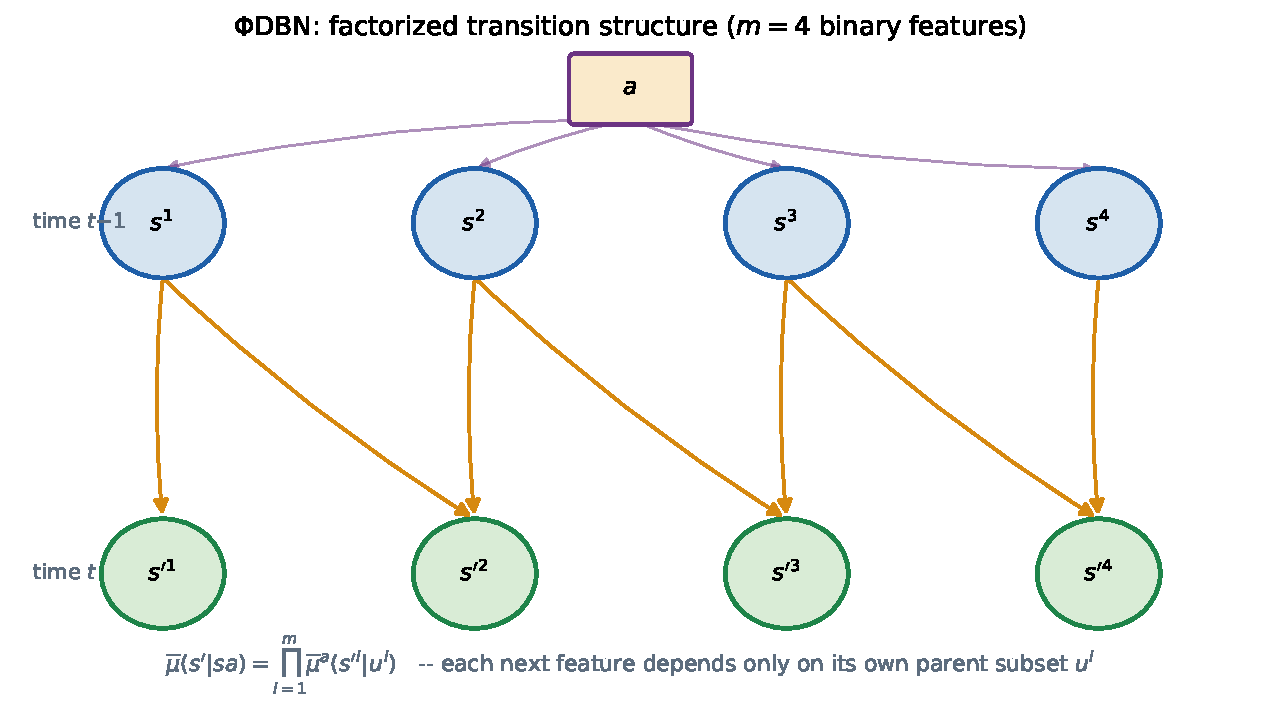
\includegraphics[width=0.72\linewidth]{dbn_factorization_schematic}

  \raggedright
  \vspace{0.3em}
  With $m=4$ binary features, each next-feature node $s'^i$ only has
  arrows coming in from its own small parent subset $u^i\subseteq\{s^1,
  \ldots,s^m\}$ (orange) and the action $a$ (purple) -- not from every
  feature of the previous state. This sparsity is exactly what keeps
  $\Phi$DBN tractable even when $m$ is large.
\end{frame}

\begin{frame}{The KT-Based Estimate}
  Since we do not know $\overline\mu^a$, we must estimate it. We could use
  frequency estimation as in $\Phi$MDP above, but instead we use the
  following \textbf{KT-based} estimate (Definition 4.1.1), which
  regularizes the counts and works better for rarely visited transitions:
  \begin{block}{KT-Based Estimate for $\Phi$DBN}
    \[
      \overline\mu^a(s^i|u^i) = \frac{|\{n\le t: u_{n-1}=u^i,\,a_{n-1}=a,\,s^i_n=s^i\}|+1/2}{|\{n\le t: u_{n-1}=u^i,\,a_{n-1}=a\}|+1}
    \]
  \end{block}
  \textbf{Plain English.} This is exactly the \textbf{Krichevsky-Trofimov
  (KT) estimator} from Chapter 4/Section 12.1: count how often feature $i$
  became $s^i$ after seeing parents $u^i$ and action $a$, add
  $\tfrac12$ (a ``pseudo-count'' that avoids ever predicting probability
  $0$ or $1$ from finite data), and divide by the total count of that
  context plus $1$.

  \vspace{0.4em}
  Using this, we estimate $\overline\mu$ and the probability of a state
  sequence $s_{1:n}$ given actions $a_{1:n}$ by
  \[
    \overline\mu(\overline h_{1:t}) = \prod_{n=1}^t \overline\mu(s_n|s_{n-1}a_{n-1})
    = \prod_{n=1}^t\prod_{i=1}^m \frac{|\{n\le t:u_{n-1}=u^i,a_{n-1}=a,s^i_n=s^i\}|+1/2}{|\{n\le t:u_{n-1}=u^i,a_{n-1}=a\}|+1}
  \]
\end{frame}

\begin{frame}[fragile]{Python: KT Estimator for a $\Phi$DBN Feature}
  We stream $8$ samples of one binary feature $s^i$ with parent
  $u^i=s^1_{t-1}$ (a single previous bit) under a constant action, and
  track how the KT estimate $\overline\mu^a(s'=1|u)$ evolves.
  \begin{lstlisting}[style=pycode]
from collections import defaultdict
data = [(0,"a",1), (1,"a",1), (1,"a",0), (0,"a",1),
        (1,"a",1), (0,"a",1), (1,"a",0), (1,"a",1)]
count_ua, count_ua1 = defaultdict(int), defaultdict(int)

def kt(u, a):
    n1, n = count_ua1[(u,a)], count_ua[(u,a)]
    return (n1 + 0.5) / (n + 1)          # KT estimate, Eq. above

for u, a, sp in data:
    pred = kt(u, a)                       # prediction BEFORE seeing sp
    count_ua[(u,a)] += 1
    if sp == 1: count_ua1[(u,a)] += 1

# Output (predictions made just before each new sample arrives):
# u=0: 0.5000 -> 0.7500 -> 0.8333  (observed s'=1 all three times)
# u=1: 0.5000 -> 0.7500 -> 0.5000 -> 0.6250 -> 0.5000
# Final estimates:
#   mu-bar^a(s'=1|u=0) = (3+1/2)/(3+1) = 0.8750
#   mu-bar^a(s'=1|u=1) = (3+1/2)/(5+1) = 0.5833
  \end{lstlisting}
  The estimate for $u=0$ climbs toward $1$ (all observed outcomes were
  $1$); $u=1$ stays near $0.5$ (mixed outcomes) -- the regularized,
  ``never fully certain'' behavior the $+\tfrac12$/$+1$ counts produce.
\end{frame}

\begin{frame}{Encoding Rewards in $\Phi$DBN}
  For the encoding of rewards we assume the reward for a next state can be
  written as the sum of functions that each depend only on an individual
  feature:
  \[
    R(s) := \sum_{i=1}^m R^i(s^i)
  \]
  This is reasonable, since we are assuming each feature of the state is
  independent of the others, and that transitions to new states/rewards
  depend only on the previous state and action. Since features
  $s^i\in\{0,1\}$, this is equivalent to a \textbf{linear function} of the
  feature vector $s\in\B^m$, for any choice of $R^i(\cdot)$:
  \[
    R(s) := w_0 + w^\top s = w_0 + w_1 s^1 + \cdots + w_m s^m
  \]
  for a suitable weight vector $w\in\R^{m+1}$. To determine if our
  weighting $w$ is good, we need a loss function comparing $R(s_t)$ to
  $r_t$ for all $s_t,r_t$ in the history. \textbf{Least squares} is a
  sensible choice, though there are many possible choices; details can be
  found in [Hut09a]. Like in Section 14.3, we combine our code lengths of
  states and rewards to find the code length of a given $\phi$:
  \[
    \mathit{Cost}(\phi|h_{1:t}) := \CL(\overline\mu(s'|s,a)|\overline h_{1:t}) + \CL(\overline\mu(r|s,a,s')|\overline h_{1:t})
  \]
\end{frame}

%% ══════════════════════════════════════════════════════════════════════════
\section{14.4 Context Tree Maximization Reinforcement Learning}

\begin{frame}{CTMRL: FRL Meets Context Trees}
  Throughout this chapter we have gone over the basics of FRL but not yet
  demonstrated it in practice. \textbf{Context Tree Maximization
  Reinforcement Learning (CTMRL)} is to FRL what MC-AIXI-CTW is to AIXI.
  CTMRL [Ngu13,NSH12] finds the \textbf{maximal context tree} and uses it
  to construct an MDP, then takes the optimal action assuming the agent is
  in that MDP.

  \vspace{0.4em}
  In Chapter 12 we saw how context trees emulate the dynamics of MDP
  environments, and that a Bayesian mixture over context trees can be done
  efficiently with \textbf{Context Tree Weighting (CTW)}: when the true
  environment was Markov, CTW performs well. In FRL we are \emph{not}
  interested in mixing over Markov environments -- instead we assume the
  true environment is \textbf{non-Markov} (completely history-dependent),
  but has some Markov encoding with an optimal feature map $\phi^*$. In
  this sense context trees are still useful: our optimal feature map
  $\phi^*$ will describe an MDP, and that MDP can be encoded as a context
  tree. \textbf{Context Tree Maximization (CTM)} is a method to choose the
  optimal $\phi$ / context tree -- recall CTM from Section 5.5 for binary
  sequence prediction; readers should familiarize themselves with that
  section first.
\end{frame}

\begin{frame}{The CTM Cost Function}
  Let $\{\kappa_1,\ldots,\kappa_{|\Ac\times\Ec|}\}=\Ac\times\Ec$ denote the
  ordered set of (action,percept) pairs. Given history $h_{1:t}$, let
  $n_{\kappa_i}$ denote the number of occurrences of $\kappa_i$ in that
  history. Let $\mathrm{P}_e^{\kappa|sa}$ denote the block probability
  estimate of seeing a sequence containing $n_{\kappa_i}$ occurrences of
  $\kappa_i$ for all $i$, given state $s$ and action $a$. Using
  $\mathrm{P}_e^{\kappa|sa}$ we build the MDP $\overline\mu$ that produces
  a state history sequence $\overline h_{1:t}$ with probability
  $\overline\mu(\overline h_{1:t}|\Sc)=\prod_{a\in\Ac}\prod_{s\in\Sc}\mathrm{P}_e^{\kappa|sa}$.
  \begin{block}{CTM Cost Function -- Eq.\ (14.4.1)}
    \[
      \mathit{Cost}(\Sc|h_{1:t}) = \log\frac{1}{\overline\mu(\overline h_{1:t}|\Sc)} + \Gamma_D(\Sc)
      = -\log\!\left(\prod_{a\in\Ac}\prod_{s\in\Sc}\mathrm{P}_e^{\kappa|sa}\right) + \Gamma_D(\Sc)
    \]
  \end{block}
  \textbf{Plain English.} $\Gamma_D(\Sc):=|\Sc|-1+|\{s:s\in\Sc,\ell(s)\neq D\}|$
  is a \textbf{model penalty} for the state set $\Sc$ relative to the
  class $\mathcal{C}_D$ of context trees of maximal depth $D$
  ($\ell(s)$ is the depth/length of context $s$). Here $s_n=\phi_\Sc(h_{1:n})$,
  with $\phi_\Sc$ extracting the suffix of $h_{1:n}$ matching a state in
  $\Sc$. This exactly matches the earlier general cost function (14.3.3).
\end{frame}

\begin{frame}{Context Tree Maximization: The Recursion}
  We rewrite $\mathit{Cost}$ so that minimizing it reduces to finding the
  \textbf{CTM tree}. From (14.4.1), maximizing $2^{-\Gamma_D(\Sc)}\overline\mu(h_{1:t}|\Sc)$
  is equivalent to minimizing $\mathit{Cost}$.
  \begin{block}{Context Tree Maximization -- Eqs.\ (14.4.2)-(14.4.3)}
    \[
      \mathrm{P}^D_{m,s} := \begin{cases}
        \frac12\max\Big\{\prod_{a\in\Ac}\mathrm{P}_e^{\kappa|sa},\;\prod_i \mathrm{P}^D_{m,\kappa_i s}\Big\} & \text{if } \ell(s)<D\\[4pt]
        \prod_{a\in\Ac}\mathrm{P}_e^{\kappa|sa} & \text{if } \ell(s)=D
      \end{cases}
    \]
    \[
      \Sc^D_{m,s} := \begin{cases}
        \bigcup_{\kappa_i}\Sc^D_{m,\kappa_is}\times\kappa_i & \text{if } \prod_a\mathrm{P}_e^{\kappa|sa} < \prod_i \mathrm{P}^D_{m,\kappa_is} \text{ and } \ell(s)<D\\
        \{\epsilon\} & \text{otherwise}
      \end{cases}
    \]
  \end{block}
  \textbf{Plain English.} At every context/node $s$ we compare two
  options: \textbf{keep} $s$ as a single state (probability
  $\prod_a\mathrm{P}_e^{\kappa|sa}$), or \textbf{split} it into its
  children $\kappa_is$ and recurse (probability
  $\prod_i \mathrm{P}^D_{m,\kappa_is}$). We take whichever is larger, times
  a $\tfrac12$ ``coding cost'' for making the choice at this node at all
  (this is exactly the same recursive idea as CTM for binary sequence
  prediction in Section 5.5, generalized to a non-binary alphabet, with
  $[\prod_a\mathrm{P}_e^{\kappa|sa}]^{-1}$ playing the role of the KT
  estimator there).
\end{frame}

\begin{frame}{Lemma 14.4.4 and Theorem 14.4.5}
  \begin{block}{Lemma 14.4.4 (Context Tree Maximization Equivalence)}
    For any state $s$, with $d=\ell(s)$, we have
    \[
      \mathrm{P}^D_{m,s} = 2^{-\Gamma_{D-d}(\Sc^D_{m,s})}\prod_{a\in\Ac}\prod_{u\in\Sc^D_{m,s}}\mathrm{P}_e^{\kappa|usa}
      = \max_{\Sc\in\mathcal{C}_{D-d}} 2^{-\Gamma_{D-d}(\Sc)}\prod_{a\in\Ac}\prod_{u\in\Sc}\mathrm{P}_e^{\kappa|usa}
    \]
    \emph{(Proof left as Exercise 4; hint: see Section 5.5.)}
  \end{block}
  Setting $s=\epsilon$ in this lemma gives the \textbf{CTM tree}, which
  minimizes the Cost function (14.4.1):
  \begin{block}{Theorem 14.4.5 (CTM Minimized Cost)}
    Given a history $h_{1:t}$, up to time $t$ we have
    \[
      \min_\Sc \mathit{Cost}(\Sc|h_{1:t}) = \log\frac{1}{\mathrm{P}^D_{m,\epsilon}(e_{1:t}|a_{<t})}
      = \log\frac{1}{\overline\mu(h_{1:t}|\Sc^D_{m,\epsilon}(h_{1:t}))} + \Gamma_D(\Sc^D_{m,\epsilon}(h_{1:t}))
    \]
  \end{block}
  \textbf{Plain English.} $\mathrm{P}^D_{m,\epsilon}$, computed at the root
  $\epsilon$ (empty context), automatically equals the best possible
  $Cost$ over every candidate $\Sc$ -- no explicit search needed.
\end{frame}

\begin{frame}[allowframebreaks]{Proof of Theorem 14.4.5}
  \textbf{Proof.}
  \begin{align*}
    \min_\Sc \mathit{Cost}(\Sc|h_{1:t})
      &= \min_\Sc \log\frac{1}{\overline\mu(\overline h_{1:t}|\Sc)}+\Gamma_D(\Sc)\\
      &= \min_\Sc \log\left(\frac{1}{\prod_{a\in\Ac}\prod_{s\in\Sc}\mathrm{P}_e^{\kappa|sa}}\right)+\Gamma_D(\Sc)\\
      &= \min_\Sc\; -\log\left(\prod_{a\in\Ac}\prod_{s\in\Sc}\mathrm{P}_e^{\kappa|sa}\right)+\Gamma_D(\Sc)\\
      &= \max_\Sc\; 2^{\log(\prod_{a\in\Ac}\prod_{s\in\Sc}\mathrm{P}_e^{\kappa|sa})-\Gamma_D(\Sc)}\\
      &= \max_\Sc\; 2^{-\Gamma_D(\Sc)}\left(\prod_{a\in\Ac}\prod_{s\in\Sc}\mathrm{P}_e^{\kappa|sa}\right)\\
      &= \mathrm{P}^D_{m,\epsilon}(e_{1:t}|a_{<t}) \qquad\blacksquare
  \end{align*}
  The last line follows from Lemma 14.4.4 with $s=\epsilon$ (so $d=0$).
  Since the recursions (14.4.2) can be computed efficiently (bottom-up,
  one pass over the tree), we now have an efficient method to find the
  optimal suffix state set $\Sc$ via (14.4.3), which minimizes the Cost
  function (14.4.1). This works well, provided the action and percept
  spaces are reasonably small for the KT-estimation to be good.
\end{frame}

\begin{frame}{Picturing the Maximizing State Set}
  \centering
  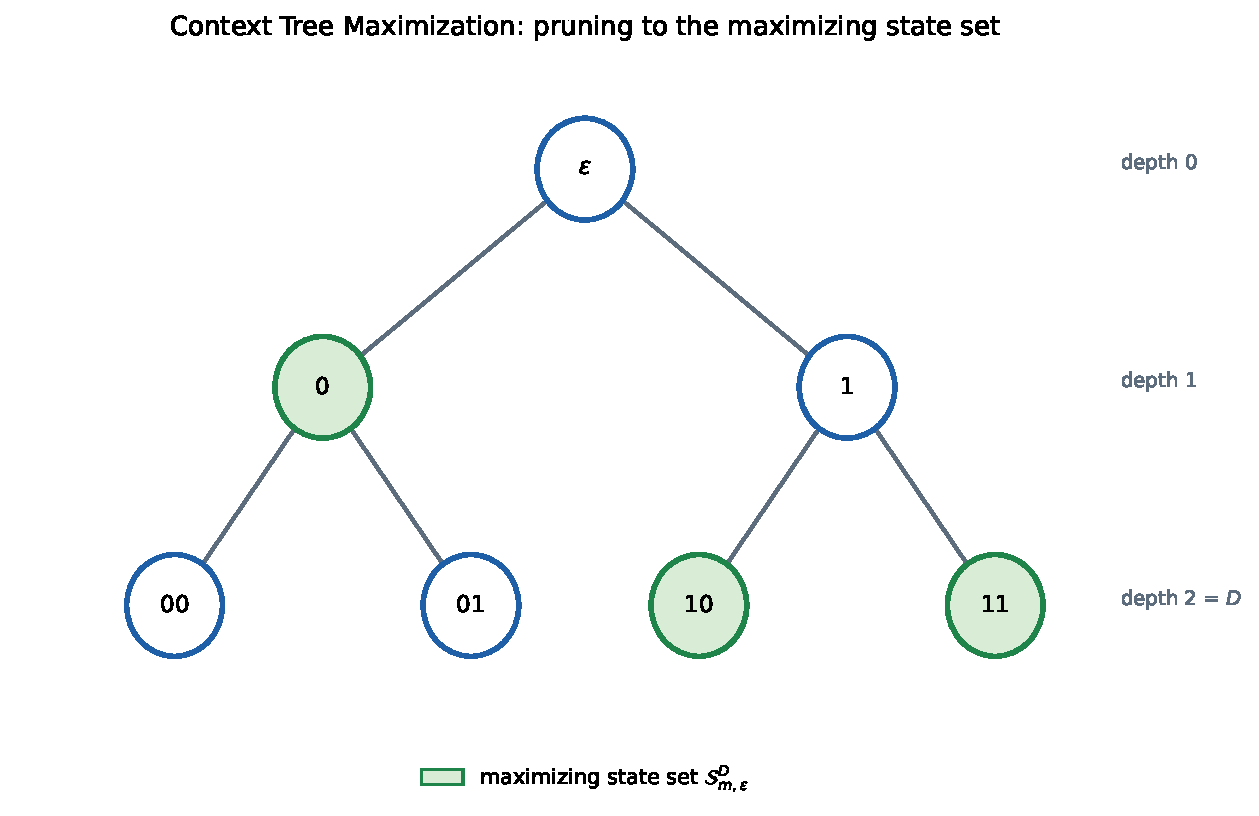
\includegraphics[width=0.6\linewidth]{ctm_tree_schematic}

  \raggedright
  At each internal node, CTM asks: ``is it worth splitting this context
  into its two children, or is this context already a good enough state
  on its own?'' Propagating that decision from leaves to root yields the
  state set $\Sc^D_{m,\epsilon}$ that exactly minimizes the Cost function
  -- the highlighted nodes above.
\end{frame}

\begin{frame}[fragile]{Python: A Toy Context Tree Maximization}
  We implement the recursion (14.4.2)-(14.4.3) directly on a depth-$2$
  binary context tree with hand-picked ``own'' block probabilities
  $\mathrm{P}_e^{\kappa|sa}$ at every node (single action, so the product
  over $\Ac$ is just one number).
  \begin{lstlisting}[style=pycode,basicstyle=\ttfamily\tiny]
import math
D = 2
own_P = {"": .05, "0": .60, "1": .60, "00": .90, "01": .50, "10": .50, "11": .90}
memo = {}

def solve(node):                                       # recursion (14.4.2)-(14.4.3)
    if node in memo: return memo[node]
    if len(node) == D:
        P, S = own_P[node], [node]
    else:
        Pc0, Sc0 = solve(node+"0"); Pc1, Sc1 = solve(node+"1")
        P, S = (0.5*Pc0*Pc1, Sc0+Sc1) if Pc0*Pc1 >= own_P[node] else (0.5*own_P[node], [node])
    memo[node] = (P, S)
    return P, S

P_root, S_root = solve("")   # at s = eps (root)

# Output:  "0": keep (P=.300);  "1": keep (P=.300);  root: SPLIT (P=.045)
#   S = ['0','1'];  -log2(P)=4.4739 bits;  Gamma_D(S)=1;  Cost=5.4739 bits
  \end{lstlisting}
  Even though every depth-2 leaf is available, CTM decides the best
  trade-off is to stop splitting at depth $1$ -- landing on exactly the
  two-state space $\Sc=\{0,1\}$ from Example 14.2.13.
\end{frame}

\begin{frame}[fragile]{Algorithm 14.3: CTMRL}
  \small
  \begin{algorithmic}[1]
    \Statex \textbf{Require:} Environment $\mu$; learning loops $m$; $n_i$'s, $n_q$; minimal percept bits $l_e$
    \State $i:=0$
    \State Create $l_e$ empty CTMs, where the $i$-th CTM predicts the $i$-th bit of the percept $e$
    \State $h:=$ initial random history by performing $n_0$ random actions;\quad $h':=h$
    \While{$i<m$}
      \State Update the $l_e$ CTMs based on history $h'$
      \State Join learned contexts from each of the CTMs to form an Action-Observation Context Tree $\Tc$
      \State Compute frequency estimates of the state transitions and reward probabilities of the MDP model based on states induced from tree $\Tc$ and history $h$
      \State Use Action-Value Iteration to find an estimate $\hat Q$ of the optimal action values based on the frequency estimates
      \State $Q:=\hat Q+\frac{R_{max}}{1-\gamma}$
      \If{$i<m-1$}
        \State $h:=\text{Q-learning}(Q,\Sc^{\Sc},\Ac,\mu,n_i)$;\quad $h:=[h,h']$;\quad $i:=i+1$
      \EndIf
    \EndWhile
    \State $\hat Q':=\text{Q-learning}(Q,\Sc^{\Tc},\Ac,\mu,n_q)$
    \State $\pi^*(s):\in\arg\max_a \hat Q'(s,a)$ for all $s\in\Sc^\Tc$
    \State \textbf{return} $\pi^*$
  \end{algorithmic}
\end{frame}

\begin{frame}{What Algorithm 14.3 (CTMRL) Does}
  $l_e$ separate CTMs handle the (binarized) percept bit-by-bit; they are
  joined into one Action-Observation Context Tree $\Tc$, which induces the
  MDP's states. $R_{max}$ is the largest possible one-step reward; adding
  $\frac{R_{max}}{1-\gamma}$ to $\hat Q$ is an \textbf{optimism bonus} that
  encourages exploring under-visited states, echoing Chapter 9's
  optimistic agents.
  \vspace{0.3em}
  \centering
  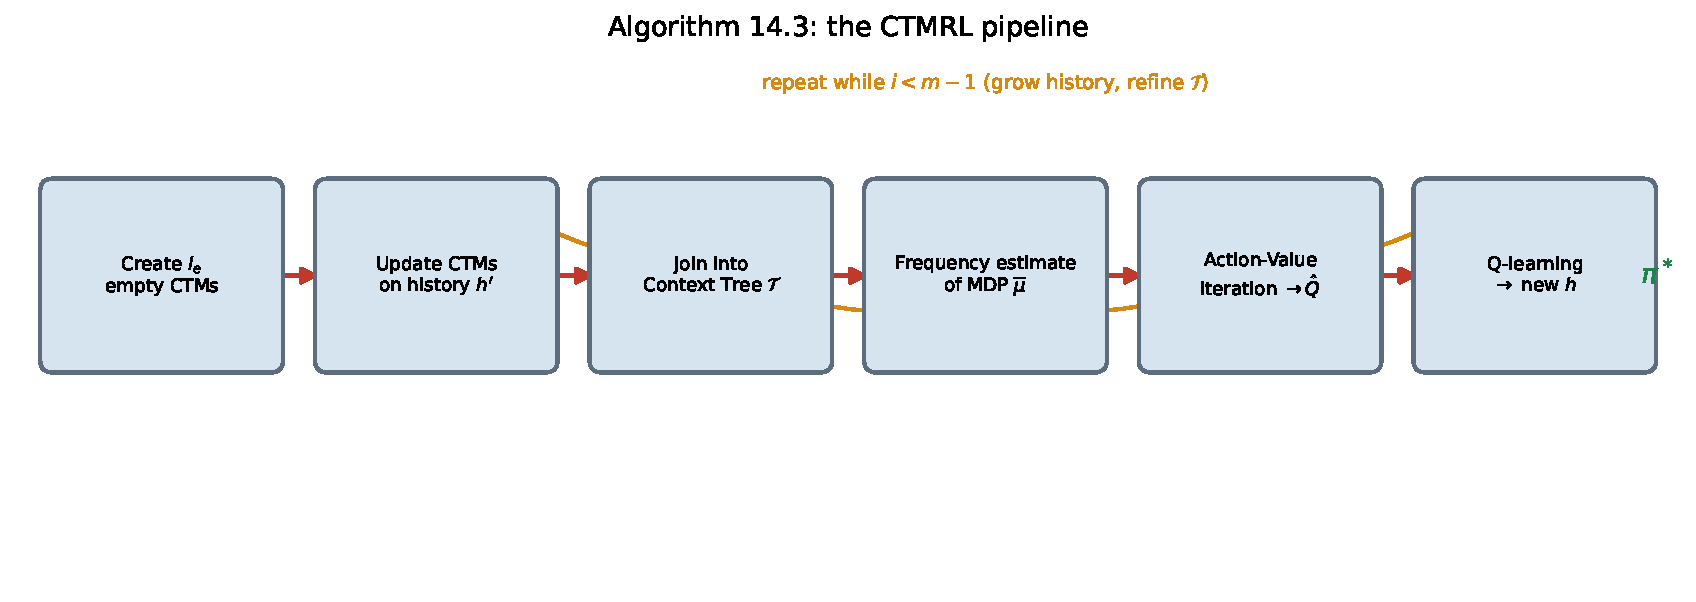
\includegraphics[width=0.85\linewidth]{ctmrl_pipeline_diagram}
\end{frame}

\begin{frame}{Binarization and CTMRL}
  For large action or percept spaces, the KT estimate will be poor. As in
  Chapter 12, we solve this by \textbf{binarizing} the action and percept
  spaces -- the same trick as before.

  \vspace{0.4em}
  Let $l_e,l_a$ be the minimum number of bits needed to describe elements
  of the percept and action space respectively. CTMRL takes as input the
  environment, a number of learning loops, $n_i$ (and $n_q$), and $l_e$.
  It starts with a CTM for each percept bit, then joins them into a
  single tree $\Tc$ containing $\Sc^{D+i-1}_{m,ae[1\ldots i-1]}$ for all
  $i\le l_e$ as subtrees. It estimates the state/reward transition
  probabilities of the MDP based on $\Tc$ via $\overline\mu$, updates the
  optimal action values with action-value iteration, then performs
  Q-learning using those values. After the learning loops complete, CTMRL
  performs Q-learning once more and defines $\pi^*(s):=\arg\max_a \hat
  Q^*(s,a)$.
\end{frame}

\begin{frame}{Comparison to AIXI and Other Agents}
  CTMRL was compared to MC-AIXI-CTW (Section 12.3), as well as other
  agents like $\Phi$MDP (Section 14.3), the classic U-Tree algorithm
  [McC96], and the more recent active LZ algorithm [FMRW10b], in a
  collection of environments detailed in Section 12.5.1. CTMRL achieved
  \textbf{comparable performance} with \textbf{drastically less
  computation time} required, with MC-AIXI-CTW taking on the order of
  \textbf{10 times} the amount of time CTMRL took to achieve similar
  near-optimal performance. This demonstrates that CTMRL is indeed a
  general, and that the FRL approach lends itself to more efficient
  approximations than AIXI approximations.
  \begin{center}
    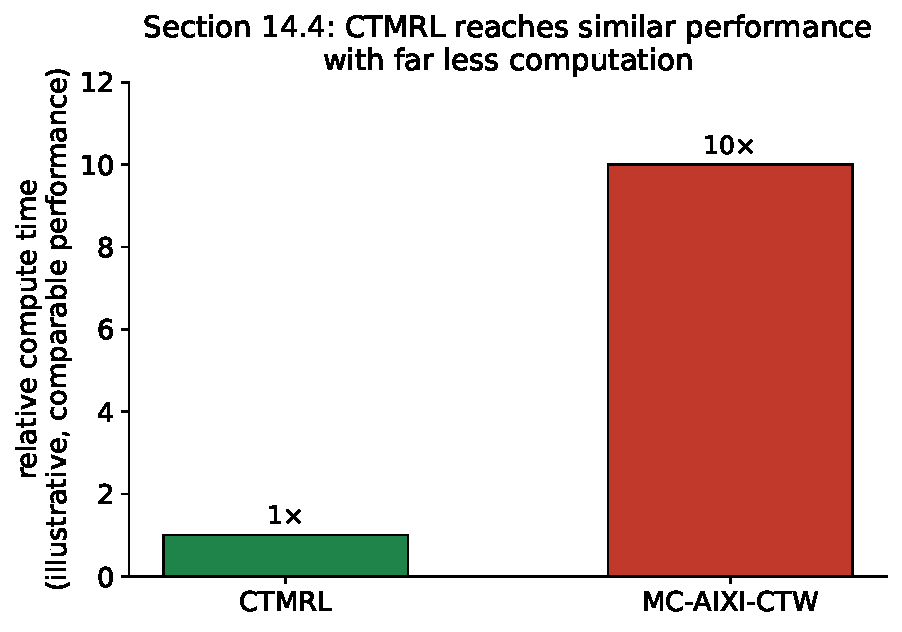
\includegraphics[width=0.35\linewidth]{ctw_vs_ctmrl_compute}
  \end{center}
\end{frame}

\begin{frame}{The AIXI vs.\ FRL/MDL Philosophy}
  The differences between CTMRL and MC-AIXI-CTW truly highlight the
  difference in approaches between the AIXI Bayesian approach and the MDL
  FRL approach:
  \begin{itemize}
    \item In the \textbf{AIXI approach}, we perform learning with
      $\xi_U\overset{\times}{=}M$ (a universal mixture that dominates the
      true measure $M$, up to a multiplicative constant) in theory, and
      \textbf{CTW} in practice; we do planning with \textbf{expectimax} in
      theory and \textbf{MCTS} in practice.
    \item In \textbf{FRL}, learning is done by finding/choosing the
      feature map $\phi$ in theory and the \textbf{maximal context tree}
      in practice (both theoretically and practically!), and expensive
      planning is replaced by \textbf{solving the MDP} via Bellman
      equations.
  \end{itemize}
  Whether explicit planning or value estimation leads to better policies
  is domain-dependent. Another potential advantage of FRL over AIXI is
  that Solomonoff's $M$ models the \emph{complete} history, which is
  expensive, while FRL only models those aspects that are separated out by
  the feature map.
\end{frame}

%% ══════════════════════════════════════════════════════════════════════════
\section{14.5 Exercises}

\begin{frame}[allowframebreaks]{Exercises}
  \begin{enumerate}
    \item \textbf{[C25]} Prove Theorem 14.2.12 (Value Inheritance).
    \item \textbf{[C25]} Prove Theorem 14.2.14 (Optimal Q-value Inheritance).
    \item \textbf{[C32]} Using binarized sequential actions to improve
      Theorem 14.2.17 to
      $|\Sc|\le O((\log|\Ac|)\varepsilon'^{-2}(1-\gamma)^{-6})$. What is the
      cost of using binarized sequential actions? The better bound
      (14.2.18) is based on deeper insights into the structure of the
      problem [MH21a]. \emph{Hint: the reason for the remaining
      logarithmic dependence on $|\Ac|$ is that the discount $\gamma$ must
      be replaced by $\gamma^{1/b}$ when $\Ac$ is sequentialized into $b$
      bits.}
    \item \textbf{[C18]} Prove Lemma 14.4.4 (Context Tree Maximization
      Equivalence).
    \item \textbf{[C35]} Implement CTMRL and compare against MC-AIXI-CTW
      in several domains.
  \end{enumerate}
  \vspace{0.5em}
  \textbf{Plain English.} The bracketed numbers $[Cxx]$ are the book's
  standard difficulty ratings (roughly, ``expect this to take about
  $xx$ minutes if you have the right background,'' scaled for
  research-level exercises).
\end{frame}

%% ══════════════════════════════════════════════════════════════════════════
\section{14.6 History and References}

\begin{frame}[allowframebreaks]{History and References}
  \textbf{Origins.} The Feature Reinforcement Learning (FRL) approach,
  using state and state-action abstractions to solve the general
  reinforcement learning problem, started with Feature MDPs
  [Hut09e,Hut09f] and Feature Dynamic Bayesian Networks (DBNs)
  [Hut09d,Hut09a]. Since its inception there has been much work along
  this line, most of which has been included in this chapter.
  Comprehensive overviews can be found in [Ngu13,DSH14a,Das16,Maj21].

  \vspace{0.4em}
  \textbf{FRL theory.} On the theoretical side, advances include using
  state abstractions for prediction and demonstrating their consistency
  [SH10]. Moving beyond the assumption that the abstracted process is an
  MDP was done in \textbf{Extreme State Aggregation} [Hut14a] (Section
  14.2). Extreme State Aggregation was extended in [MH21b,MH21a], which
  binarized the action space to gain a double-exponential improvement on
  a bound on the required state space size. Action-state abstractions
  were investigated in [MH19], where the authors showed when the
  state-action abstraction can lead to near-optimal performance. The
  sequel to the original FRL papers [Hut09d,Hut09a] extended [Hut09e,Hut09f]
  to more complex structured/factored MDPs, specifically focusing on
  DBNs. [RLDG22] introduces a method able to give PAC guarantees in the
  episodic setting, assuming there exists a Markov abstraction.

  \framebreak

  \textbf{FRL practice.} On the practical side, advances include using a
  practical implementation of $\Phi$MDP to achieve performance
  competitive to MC-AIXI-CTW [NSH11], FRL with Context Tree Maximization
  [NSH12] (Section 14.4), FRL with looping suffix trees to solve the
  long-term dependency problem [DSH12], studying Q-learning in the
  general reinforcement learning setting [DSH13,MH18], and extending
  MC-AIXI-CTW by using state abstractions on the history [YZWN22]. Code
  for the approximations presented in this chapter is available from the
  book's website \texttt{hutter1.net/ai/uaibook2.htm}.

  \vspace{0.4em}
  \textbf{Regret results.} There are many ways to measure the performance
  of an agent or abstraction; one is with \textbf{regret} (Section
  8.1.4). In [MMR11] the authors introduced an algorithm for the FRL
  setting achieving regret $O(T^{2/3})$. This bound was improved when
  [NOR13] proposed an algorithm achieving regret $O(T^{1/2})$, which is
  optimal at least asymptotically. Both prior approaches relied on being
  given a finite set of abstractions, but [NMRO13] extended this to a
  countably infinite set. Many approaches consider \emph{exact}
  abstractions; [OMR14] derived results for \emph{approximate}
  abstractions, and [OPL+19] introduced a new algorithm achieving
  comparable regret bounds with possibly better bounds depending on the
  effective size of the induced state space.

  \framebreak

  \textbf{Solving MDPs with state abstractions.} FRL focuses on solving
  the general RL problem through state abstractions; there is also much
  work on solving simpler MDP (and POMDP) problems this way. [SLO22]
  surveys many model-based methods for this problem. [LWL06] began the
  process of comparing five different unification approaches. Approximate
  abstractions are studied in [AHL16]. Continual/life-long learning faces
  an ever-growing history; state abstractions help alleviate this
  [AALL18]. Rate distortion theory was used in [AAA+19] to make the
  compression/value trade-off explicit. When the \emph{action} space is
  very large, state-\emph{action} abstractions are natural [MH19,AUK+20].
  On the practical side, an exploration strategy based on feature
  representations gave state-of-the-art performance in Atari [MSEH17],
  and state abstractions reduced the size of sample-based search
  [HFD17].

  \framebreak

  \textbf{Classical reinforcement learning.} A general introduction to
  classical state-based RL can be found in [SB18] (see Section 6.9 for
  more advanced books). It covers multi-armed bandits (Section 12.2.3),
  finite MDPs (Chapter 11), Bellman equations (Section 14.1), MCTS
  planning (Section 12.2.4), TD($\lambda$) [Sut88,HL07], Q($\lambda$)
  [WD92,PW94,DSH13,MH18], SARSA [RN94], approximation methods, policy
  gradients [Wil92,KHS01a], applications, and dichotomies: off- vs.\
  on-policy, exploration vs.\ exploitation, model-based vs.\ model-free.

  \vspace{0.4em}
  \textbf{Other RL ideas.} The most widely used abstractions in RL are not
  discrete state/history aggregations, but approximations based on
  continuously parameterized (Q-)Value functions. Even for \emph{linear}
  function approximation, convergence is hard to come by: model-free
  TD-style algorithms cannot be guaranteed to converge to the correct
  solution unless the linear basis functions are essentially state
  aggregators [HYZM19]. Model-based methods and brilliant ``unnatural''
  algorithms like ETD [SMW16] have convergence guarantees for linear
  function approximation. For state aggregation, [MH18] shows Q-learning
  converges even if the aggregated dynamics is non-Markov, as in Section
  14.2. [HL07] derives a unique state-dependent learning rate for
  TD($\lambda$) via a variational principle and bootstrapping.

  \framebreak

  Rather than hard aggregation or smooth function approximation, one can
  also impose or use a \textbf{metric} on the observation or state space,
  natural in RL for robotics [Thr02]. [ZGHS06] extends [McC96] to general
  metrics over histories and hence continuous POMDPs, with an RL algorithm
  that learns directly on a mobile robot.

  \vspace{0.4em}
  An unorthodox RL approach is to learn the sequence of actions most
  likely to cause the agent to transition from state $s$ to $s'$ -- these
  \textbf{inverse MDP models} automatically only model the
  action-relevant aspects of the world [HH22]. With this idea in mind,
  [OHC+20] presented a method to meta-learn the update rule used, instead
  of a fixed update rule. \textbf{Imagination-based planning} was
  introduced in [PLV+17] to let agents construct and evaluate plans
  without taking real actions; an alternative imagination approach was
  studied in [SvHH+16], which learned a model for planning purposes only
  (with possibly different state, action, reward space, and time steps).

  \framebreak

  In [OIO19] a simple way to interpret RL as inference was established.
  \textbf{Distributional RL} [BDM17,BDR23,WDA+23] uses Bellman equations
  [Bel57] for the \emph{distribution} of returns, and argues why this
  improves performance even when we only care about expected returns.
  Related is \textbf{Upside-down RL} [Sch19a]. RLAdvice [DSH14b] is an
  imitation learning algorithm based on (Bayesian) DAgger, using value
  estimates from UCT as advice, applied to three Atari games from the
  Arcade Learning Environment (ALE).

  \vspace{0.4em}
  \textbf{Other AGI approaches.} There are many approaches to building
  artificial general intelligences [GP07,AGI08], with [SBP22,LeC22] two
  prominent recent examples.
\end{frame}

\end{document}
